%% teaser

\includepdf{imgs/sneeze-sequence.pdf}

\iffalse
\begin{frame}

  \frametitle{But what are \textit{droplets}?}

  \bigskip \bigskip
  \begin{columns}[T]
    
    \begin{column}{0.38\textwidth}
      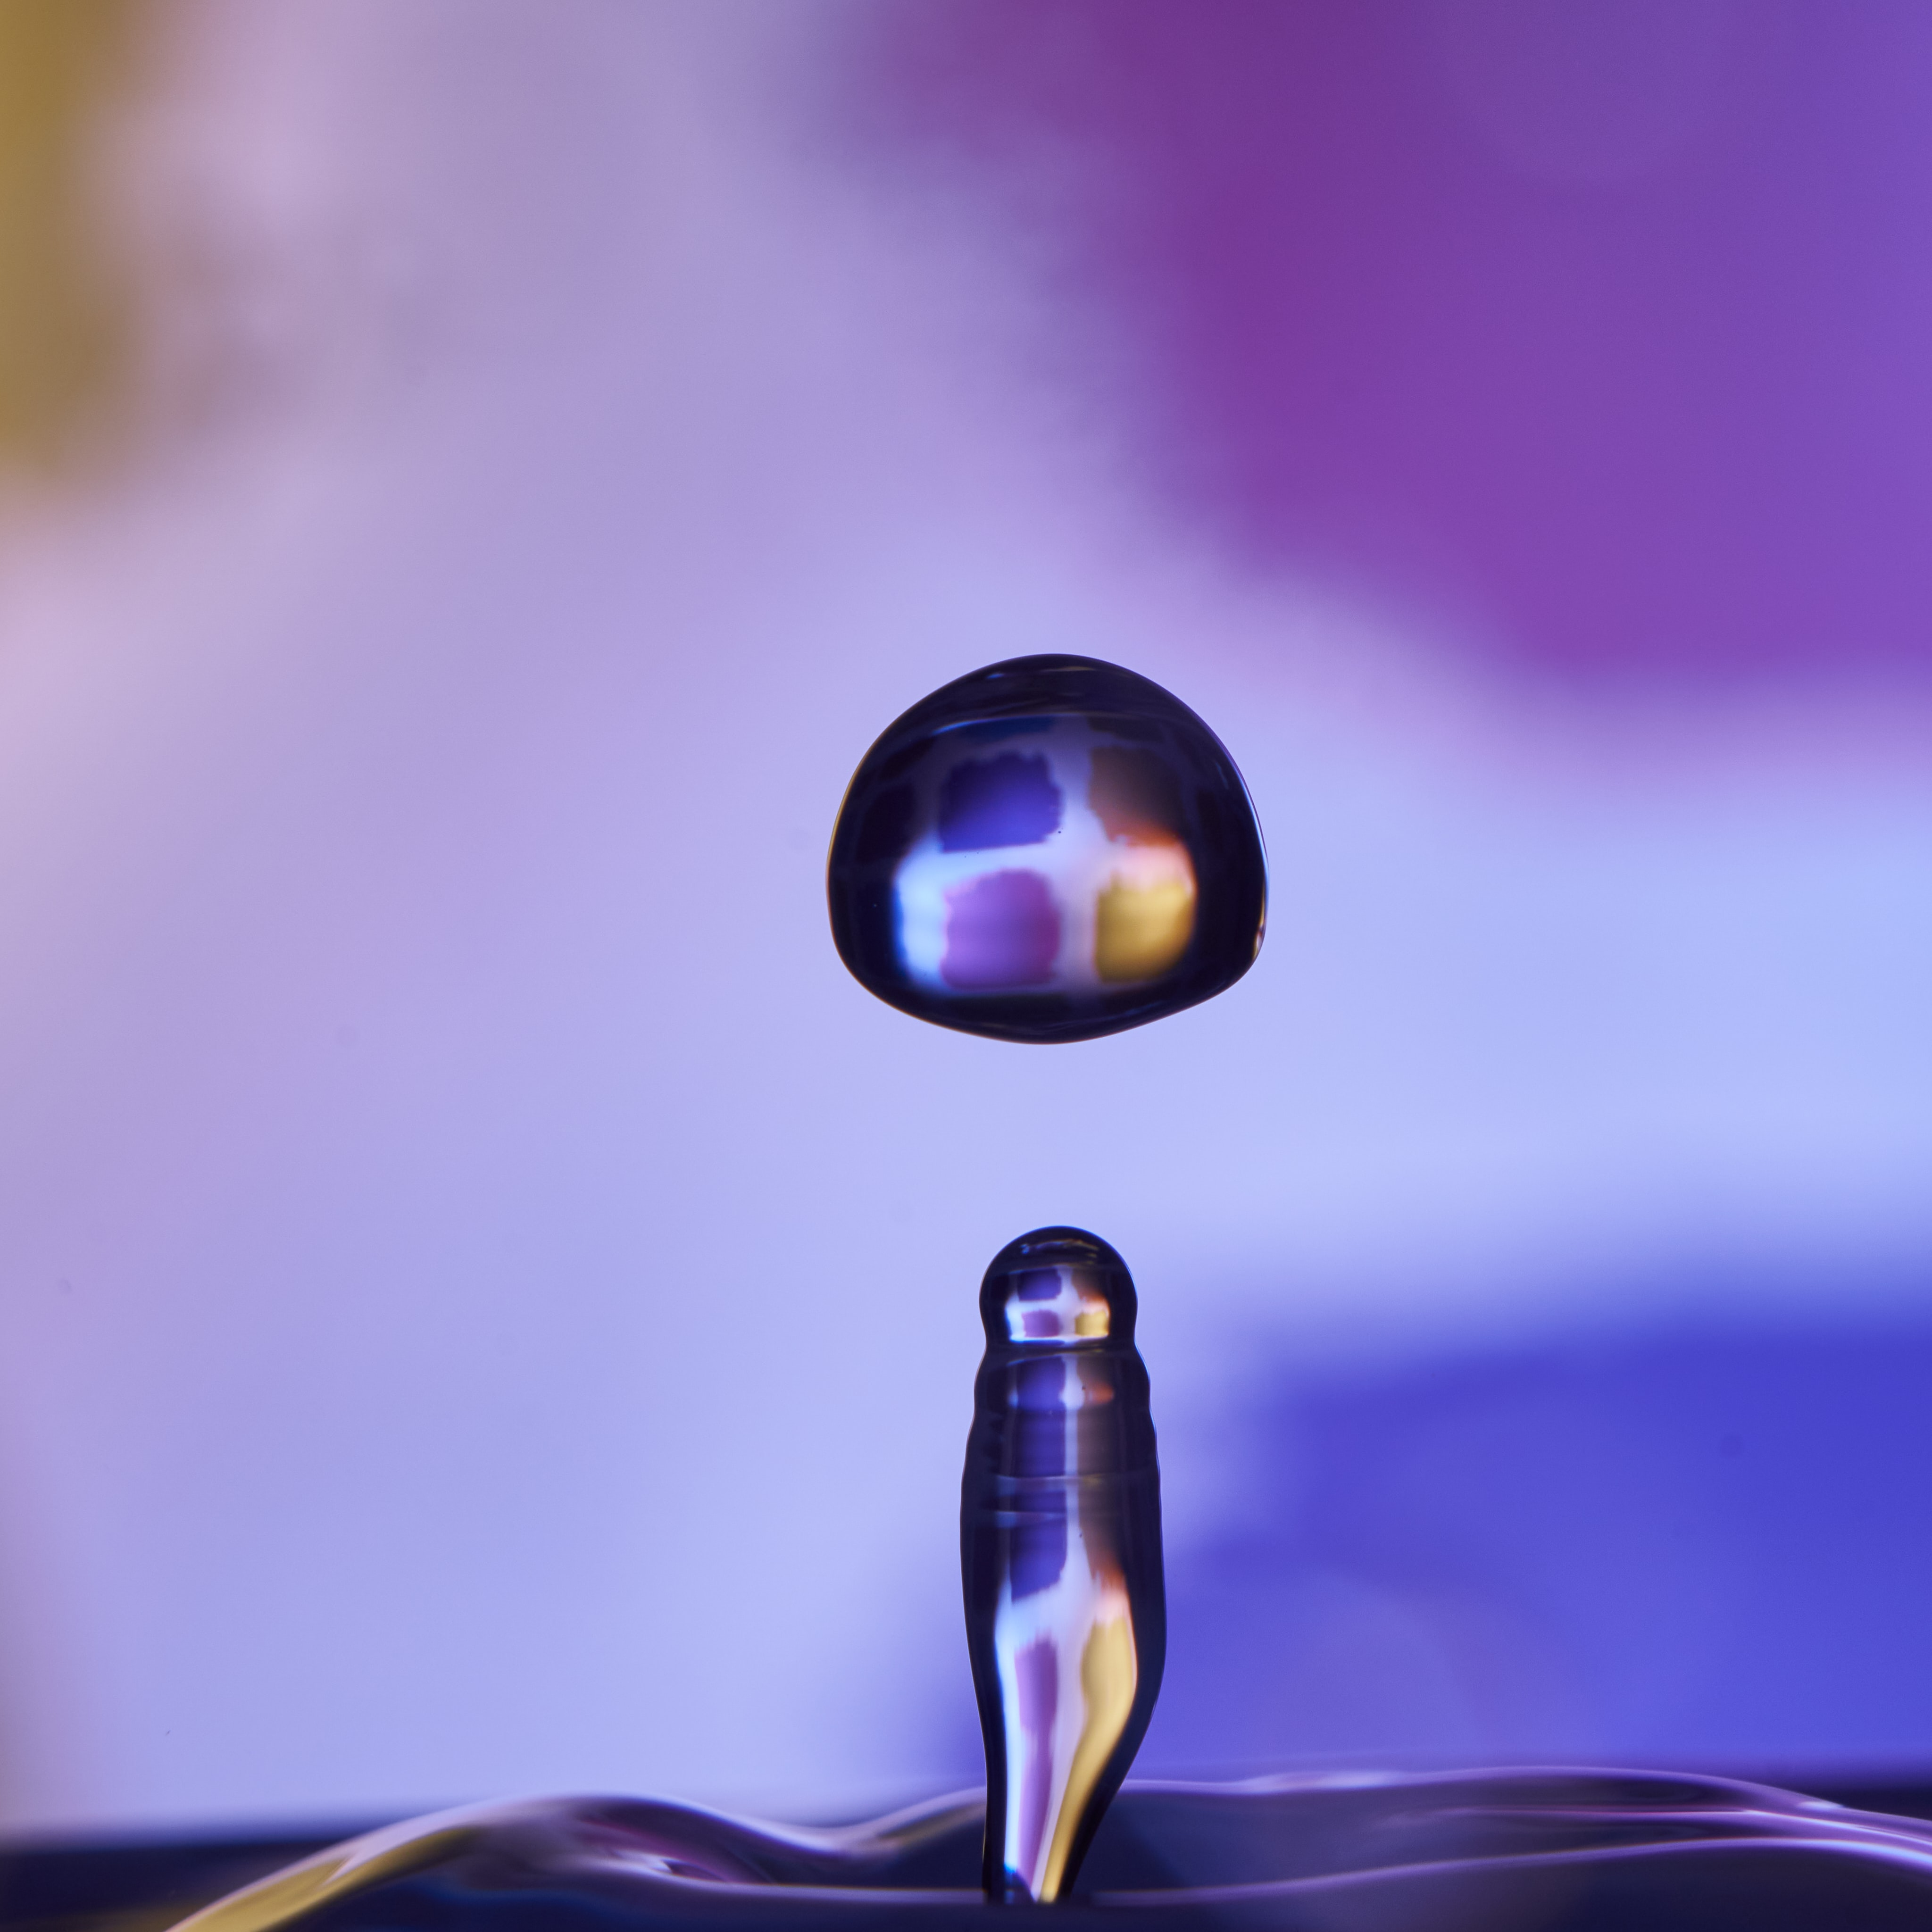
\includegraphics[height=4.8cm]{imgs/droplet_martin-brechtl-unsplash.png}
      \vskip.3cm
      Droplets are micron to millemetre sized liquid balls formed under surface tension.%
      \footnote<.->[frame]{Photo by Martin Brechtl on Unsplash.}
    \end{column}

    \pause
    \begin{column}{0.45\textwidth}
      \movie[showcontrols]{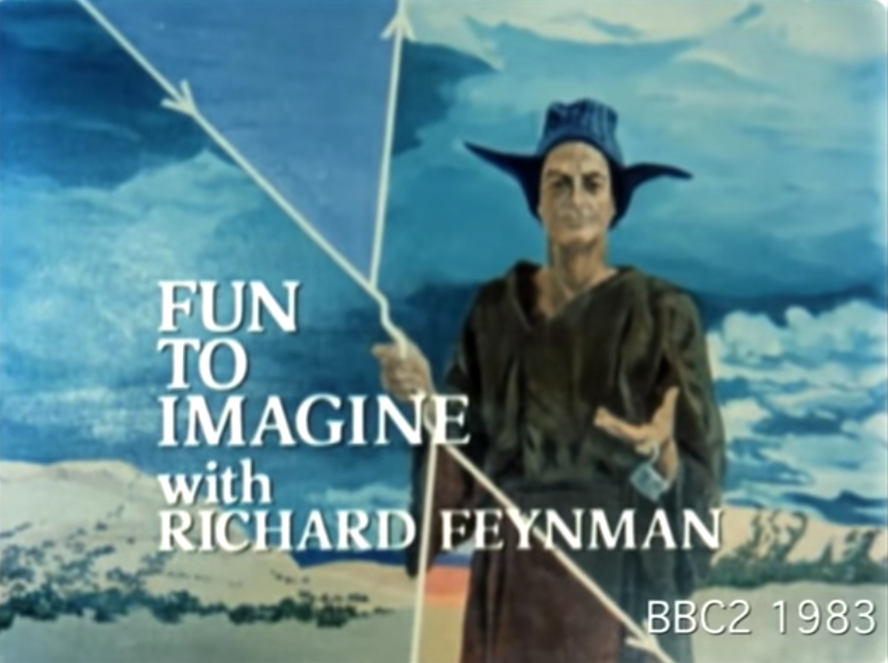
\includegraphics[height=4.8cm]{imgs/St_Feynman.png}}
            {videos/droplet-Feynman.mp4}
      \vskip.3cm
      BBC interview of Richard Feynman (1983).%
      \footnote<.->[frame]{Source: \texttt{https://youtu.be/P1ww1IXRfTA}.}
      
      \pause
      \vskip.3cm
      %\centering
      \textcolor{bb}{\bf Droplets are fun subjects!}
    \end{column}
  \end{columns}

\end{frame}
\fi


%% outline
\begin{frame}{Outline}
  \protect\hypertarget{outline}{}
  \tableofcontents
\end{frame}

%%
\hypertarget{part1}{%
  \section{Part I: Fabricating Photonic Crystals (PhC)}}

%% 
\hypertarget{background1}{%
  \subsection{Background, motivation and challenge}}

\begin{frame}
  \frametitle{Background, motivation and challenge}

  \emph{Photonic crystals} (PhC) are materials patterned with a periodicity in dielectric constant
  and show great potential for building sophisticated optical circuitry that can
  route, filter, store or suppress optical signals.
  \bigskip
  
  \begin{columns}[T]
    
    \begin{column}{0.6\textwidth}
      \begin{figure}
        \centering 
        \includegraphics[height=4.8cm]{imgs/photonic_crystal_fibre.png} 
        \caption{A scanning electron micrograph of a solid-core photonic crystal fibre and its far-field optical pattern.%
          \footnote<.->[frame]{P. Russell, Science: 358-362. (2003)}
          \textcopyright \enspace AAAS Science.}
      \end{figure}
    \end{column}
    \hskip0.5cm
    \pause
    \begin{column}{0.3\textwidth}
      \begin{figure}
        \centering 
        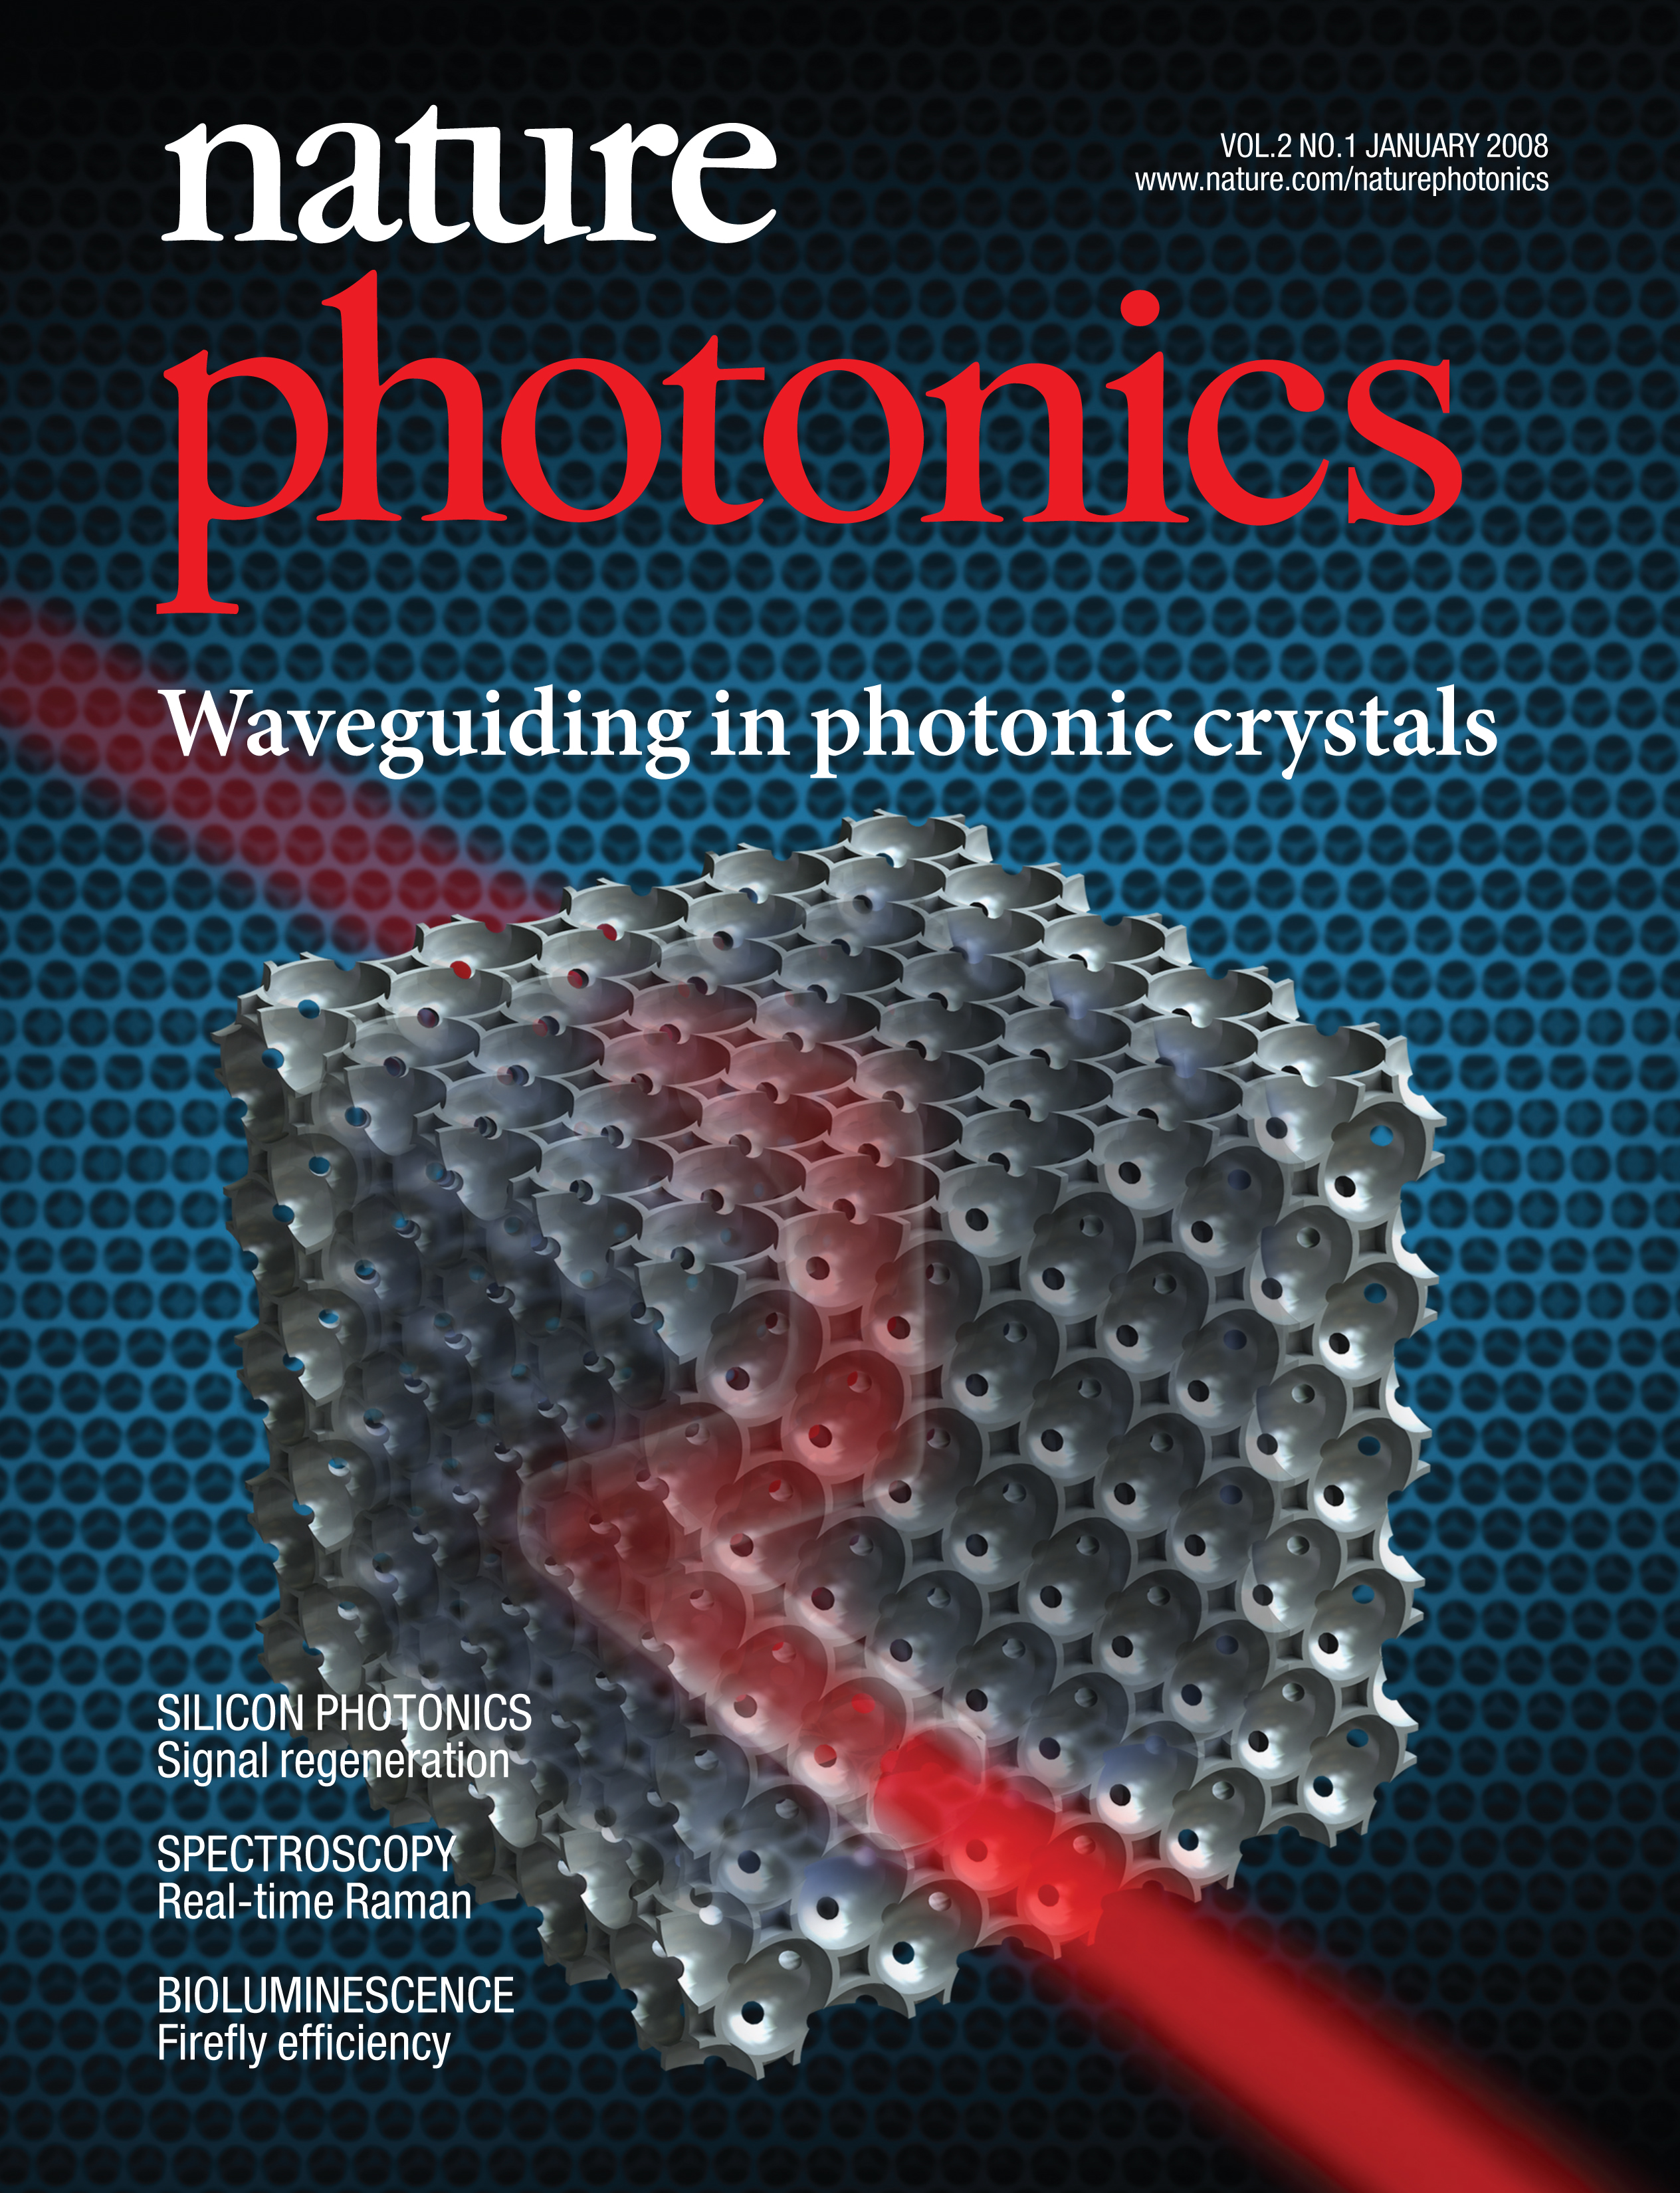
\includegraphics[height=4.8cm]{../imgs/photonics_cover.jpg} 
        \caption{An artistic rendering of a light beam passing through a 3D photonic crystal.
          \textcopyright \enspace Springer Nature (2008).}
      \end{figure}
    \end{column}
  \end{columns}
  
\end{frame}

\begin{frame}
  \frametitle{Background, motivation and challenge}

  \begin{textblock}{145}(5,12)
    Despite the theoretical promise, fabricating photonic crystals with 3D bandgaps is challenging in practice.
  \end{textblock}

  \begin{textblock}{145}(5,20)
  \begin{columns}[T]
    \begin{column}{0.45\textwidth}
      \begin{figure}
        \centering
        \includegraphics[height=4.8cm]{imgs/diamond-111.png}
        \caption{A diamond cubic (view angle 111), ideal structure of PhC.}
      \end{figure}
    \end{column}

    \only<2->{
      \begin{column}{0.45\textwidth}
        \begin{figure}
          \centering
          \includegraphics[height=4.8cm]{imgs/patchy_colloid.png}
          \caption{Self-assembly of micron-sized patchy particles mimicking the arrangements of bonds around atoms.%
            \footnote<2->[frame]{Wang \etal Nature. 491, 51-55(2012).}
            \textcopyright \enspace Springer Nature (2012).}
        \end{figure}
      \end{column}
    } % end only
    
  \end{columns}
  %\vskip0.1cm
  
  %\pause
  \centering{
    \only<3->{\xb{\bf The obtained clusters may serve as basic building blocks for fabricating PhC.}}
    \vskip0.08cm
    %\pause
    \only<4->{\xr{\bf The challenge is to speed up the process.}}}
  \end{textblock}

\end{frame}

%%
\hypertarget{experiment}{%
  \subsection{Experiments, strategy and questions}}

\begin{frame}[t]
  \frametitle{Experiments, strategy and questions}

  A few years ago, a series of experiments performed at ESPCI, Paris suggested a possible solution.%
  \footnote{B. Shen \etal Exp. Fluids, 55, 1. (2014); B. Shen \etal Adv. Sci., 3: 1600012. (2016).}
  
  \begin{textblock}{80}(8,21)    
    \movie[showcontrols]{\includegraphics[height=3cm]{imgs/espci-delta.png}}{videos/espci-3drops.mp4}
  \end{textblock}
  \begin{textblock}{80}(8,51)    
    \movie[showcontrols]{\includegraphics[width=6.5cm]{imgs/espci-tetra.jpg}}{videos/espci-4drops.mp4}
  \end{textblock}
  \begin{textblock}{80}(78,21)    
    \includegraphics[height=4.6cm]{imgs/espci_clusters.png}
  \end{textblock}
  \begin{textblock}{135}(8,71)    
    Figure: (a) Assembly of two to four droplets in a microfluidic chip.
    (b-e) Electron micrographs of clusters of various shapes; scale bars: 10 $\mu$m.
    Images courtesy of Joshua Ricouvier.
  \end{textblock}

  \begin{textblock}{135}(6,81)  
    \only<2->{\xb{\bf Here, the droplet assembly is driven by the flow. Hence, it is much faster.} \vskip0.05cm}
    \only<3->{\xr{\bf The questions are why do they organize into such patterns and can we further optimize it?}}
  \end{textblock}
  
\end{frame}

%%
\hypertarget{dipolar}{%
  \subsection{A simple q2D dipolar model}}

\begin{frame}
  \frametitle{A simple q2D dipolar model}

  \begin{textblock}{148}(5,12)
    Noticing the geometric confinement of the microfluidic channel, researchers at ESPCI proposed the following \emph{dipolar model}.
  \end{textblock}

  \begin{textblock}{148}(5,19)
    \begin{columns}[T]
      
      \begin{column}{0.45\textwidth}
        \vskip0.2cm
        \centering
        \only<1-5,7,8>{\includegraphics[height=4cm]{imgs/espci-chip-cartoon.png} \vskip.3cm}
        \only<2-5>{\includegraphics[height=1.6cm]{imgs/espci-pancake.png}}
        \only<3-5>{\includegraphics[height=1.9cm]{imgs/espci-depletion.png}}
        \only<6>{\vskip.5cm 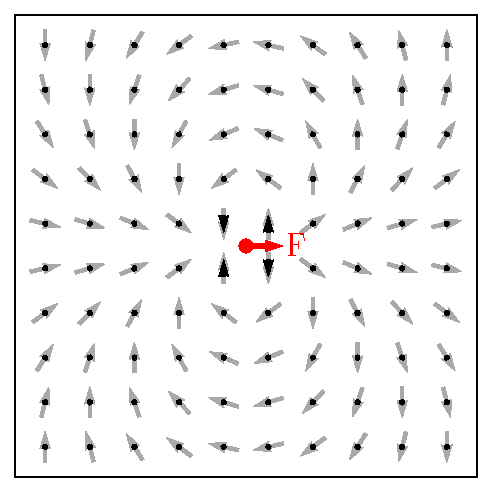
\includegraphics[height=6cm]{../imgs/dipolar.pdf}}
        \only<7->{\includegraphics[height=2.8cm]{imgs/espci-dipolar-cartoon.png} \\}
        \only<8>{\xr{\bf Is this picture really correct?}}
      \end{column}
      
      \begin{column}{0.45\textwidth}
        \only<2->{
          \begin{bluecolorbox}[Hypotheses]
            \begin{itemize}
            \item Droplets obey laws in quasi-two- dimensional (q2D) space.
              \only<3->{\item Depletion force attracts nearby drops.}
              \only<4->{\item Hydrodynamic interactions (HI) lead to the rearrangement dynamics.}
            \end{itemize}
          \end{bluecolorbox}
        } %end only
        \vskip.2cm
        \only<5->{
          \begin{bluecolorbox}[Equations of motion (due to HI)]
            \begin{equation} \notag
              \begin{aligned}
                & {\bm u}^\infty(x,y,z) \approx -\frac{z(H-z)}{2\mu} \nabla p(x,y), \\
                & \delta{\bm u}_{ij} = {\bm B}_{ij} {\bm F}_j, \quad {\bm U}_i = {\bm u}^\infty_i + \sum_{j \ne i} \delta{\bm u}_{ij},
              \end{aligned}
            \end{equation}
            where
            \begin{equation} \notag
              \begin{aligned}
                {\bm B}({\bm x}) \approx -\frac{\alpha H}{\mu} \bigg( \frac{{\bm I}}{\abs{\bm x}^2} -
                \frac{ 2{\bm x}{\bm x} }{ \abs{{\bm x}}^4} \bigg).
              \end{aligned}
            \end{equation}
          \end{bluecolorbox}
        } % end only
      \end{column}

    \end{columns}
  \end{textblock}
  
\end{frame}

%%
\hypertarget{simulation1}{%
  \subsection{3D numerical simulations}}

\begin{frame}
  \frametitle{3D numerical simulations}

  To investigate the hydrodynamics, we set up direct numerical simulations of droplets in microchannels.
  \vskip0.3cm

  \pause
  \begin{columns}[T]

    \begin{column}{0.55\textwidth}
      \begin{bluecolorbox}[Mathematical formulation]
        The incompressible Navier-Stokes (NS) equations read,
        \begin{subequations} \label{eq:Navier-Sotkes}
          \begin{equation}
            \nabla \cdot {\bm u} = 0,
            \label{eq:div-free}
          \end{equation}
          \begin{equation}
            \rho \bigg(\frac{\partial {\bm u}}{\partial t} + {\bm u} \cdot \nabla {\bm u} \bigg) = \nabla \cdot {\bm \sigma} + {\bm f},
            \label{eq:NS}
          \end{equation}
        \end{subequations}
        where $\bm \sigma$ is the viscous stress tensor, given as
        \begin{equation}
          \begin{aligned}
            {\bm \sigma} = -p {\bm I}+ \mu \bigg( \nabla {\bm u} + (\nabla {\bm u})^T \bigg),
          \end{aligned}
        \end{equation}
        and is subject to the following boundary condition across the interface
        \begin{equation} \label{eq:stress-bc}
          ({\bm \sigma}_+ - {\bm \sigma}_- ) \cdot {\bm n} = \gamma \kappa {\bm n} - \nabla \gamma.
        \end{equation}
      \end{bluecolorbox}
    \end{column}

    \pause
    \begin{column}{0.4\textwidth}
      \centering
      \begin{bluecolorbox}[Non-dimensional numbers]
        \begin{equation} \notag
          \begin{aligned}
            \textrm{Re} = \frac{\rho UL}{\mu}, \quad
            \textrm{Ca} = \frac{\mu U}{\gamma}, \quad
            \textrm{Fr} = \frac{U^2}{FL}.  
          \end{aligned} \medskip
        \end{equation}
      \end{bluecolorbox}
      \vskip0.2cm

      \pause
      \begin{flushleft}
        In the experiments, %Re $\sim 10^{-2}$, Ca $\sim 10^{-5}$, Fr $\sim 10^{-5}$,
        \begin{equation} \notag
          \begin{aligned}
            \textrm{Re} \sim 10^{-2}, \quad
            \textrm{Ca} \sim 10^{-5}, \quad
            \textrm{Fr} \sim 10^{-5}.  
          \end{aligned}
        \end{equation}
        It means that inertial effects are negligible,
        the droplets will remain mostly spherical,
        and gravity matters.
        \vskip0.4cm

        \pause
        The rest of the task is to develop a solver that can solve these equations accurately.
      \end{flushleft}
    \end{column}
    
  \end{columns}
  
\end{frame}

%%
\hypertarget{icls}{%
  \subsubsection{ICLS/GFM}}
%%1
\begin{frame}[t]
  \frametitle{Interface-resolved one-fluid methods}

  \begin{columns}[T]

    \begin{column}{0.45\textwidth}
      \vskip0.2cm
      \only<1-4>{
      There are numerous methods for direct simulation of droplets in fluids, such as
      \medskip
      \begin{itemize}
      \item front-tracking methods
      \item volume-of-fluid methods    
      \item level set (LS) methods
      \item phase field methods
      \item lattice-Boltzmann methods
      \item boundary integral methods
      \item ...
      \end{itemize}
      } % end only
      \medskip
      \only<2-4>{We use {\bf LS} for its simplicity and mathematical convenience.}

      \medskip
      \only<4>{However, there is an \xr{issue}...}
      \only<5->{\movie[showcontrols,poster,width=6cm,height=6.5cm]{}{videos/serpentine.mp4} \vskip0.2cm}
      \only<6->{\hskip1.2cm \xr{\bf LS is not mass-conserving.}}
      
    \end{column}

    
    \begin{column}{0.5\textwidth}
      \only<3->{
      \begin{bluecolorbox}[Classical LS formulation]

        The level set function, $\phi$, is defined as the signed distance to the interface $\Gamma$,
        \begin{equation} 
          \phi({\bm x}) = sgn({\bm x}) |{\bm x}-{\bm x}_\Gamma|.
        \end{equation}
        For example, a sphere of radius $r$ centered at origin can be represented as
        \begin{equation} \notag
          \Gamma = \{ {\bm x} ~ \rvert ~ \phi({\bm x}) = 0 \},
        \end{equation}
        where
        \begin{equation} \notag
          \phi({\bm x}) = |{\bm x}| -r.
        \end{equation}
        Knowing $\phi$, the normal and the curvature of the interface can be readily calculated as
        \begin{equation}
          {\bm n} = \nabla \phi / \abs{ \nabla \phi }, \quad \kappa = \nabla \cdot {\bm n}.
        \end{equation}
        The motion of the interface is captured by
        \begin{equation} \label{eq:ls-avd}
          \frac{\partial \phi}{\partial t} + \bm{u} \cdot \nabla \phi = 0.
        \end{equation}
        
      \end{bluecolorbox}
      } %end only
    \end{column}
    
  \end{columns}

\end{frame}
%%2
\begin{frame}[t]
  \frametitle{Interface-correction level set/ghost fluid method (ICLS/GFM)}
  
  \begin{columns}[T]

    \begin{column}{0.45\textwidth}
      \vskip0.2cm
      \only<1->{
      To remedy the problem, we developed a simple mass-correction scheme.%
      \footnote<.->[frame]{Z. Ge \etal J. Comput. Phys. 353: 435-459. (2018)}
      } % end only
      \vskip0.2cm
      \only<2->{
      The key idea is to construct a correction-velocity, ${\bm u}_c$,
      such that the total volume is controlled by doing an additional advection.
      \vskip0.2cm} % end only
      \only<4>{\centering{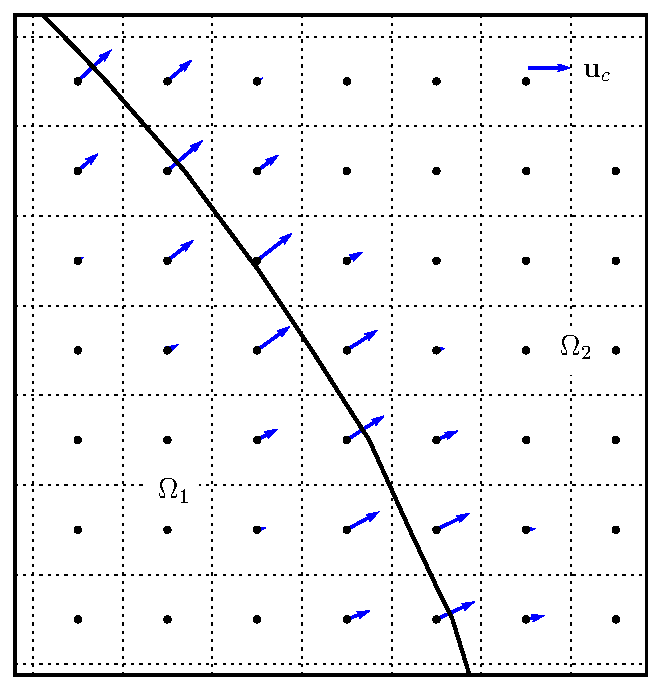
\includegraphics[width=0.75\textwidth]{../paper1/Figures/mc.pdf}}} % end only
    \end{column}

    
    \begin{column}{0.5\textwidth}
      \only<3->{
      \begin{bluecolorbox}[ICLS formulation]

        The level set is defined and evolved in the same way as in the classical formulation,
        except that we also periodically examine the fluid mass loss, $-\delta V/\delta t$.
        This allows us to define ${\bm u}_c$ from
        \begin{equation} \notag
          \int_\Gamma {\bm n} \cdot {\bm u}_c \,d\Gamma = \frac{\delta V}{\delta t}.
        \end{equation}
        If ${\bm u}_c$ is known, then solving
        \begin{equation}
          \frac{\partial \phi}{\partial t} + {\bm u}_c \cdot \nabla \phi = 0,
        \end{equation}
        will remove the mass loss accumulated over $\delta t$.

        It can be shown that
        \begin{equation}
          {\bm u}_c(\phi) = \frac{\delta V}{\delta t} \frac{\kappa(\phi)}{A_f} \delta_\epsilon (\phi),
        \end{equation}
        where $A_f = \int_\Gamma f_s \delta_\epsilon (\phi)|\nabla \phi| \,d\Gamma$.
        
      \end{bluecolorbox}
      } %end only
    \end{column}
    
  \end{columns}

\end{frame}
%%3
\begin{frame}[noframenumbering,t]
  \frametitle{Interface-correction level set/ghost fluid method (ICLS/GFM)}

  To verify, we simulate the deforming circle, same as before.
  \vskip0.2cm
  \centering
  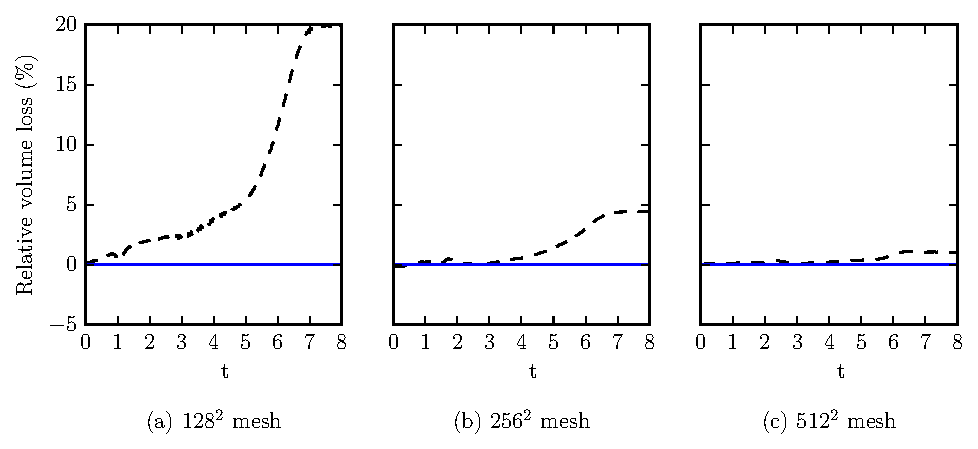
\includegraphics[width=0.8\textwidth]{../paper1/Figures/serp_loss.pdf}
  \vskip0.3cm
  \pause
  \xb{\bf A global mass conservation is now achieved.}

\end{frame}
%%4
\begin{frame}[t]
  \frametitle{Interface-correction level set/ghost fluid method (ICLS/GFM)}

  The coupled flow solver also requires accurate computation of surface tension and a hydrodynamic model to impose the depletion force.

  \only<2>{
    \begin{textblock}{130}(5,23)
      \begin{algorithm}[H] \notag
        %\xb{\footnotesize //time marching} \\
        \For{$n=1,2,\dots,N$}{
          %\xg{\footnotesize //level set advection} \\
          $\phi^1 = \phi^{(n)} + \Delta t \cdot {AD}(\phi^{(n)})$ \\
          $\phi^2 = \frac{3}{4} \phi^{(n)} + \frac{1}{4} \phi^1 + \frac{1}{4} \Delta t \cdot {AD}(\phi^1)$ \\
          $\phi^{(n+1)} = \frac{1}{3} \phi^{(n)} + \frac{2}{3} \phi^2 + \frac{2}{3} \Delta t \cdot {AD}(\phi^2)$ \\
          
          %\xg{\footnotesize //correct and reinitialize the level set every $N_i$ steps} \\
          \If{$n \mod N_i =0$}{
            {\small advect with ${AD}(\phi) = (\delta V/\delta t) (\kappa \delta(\phi)/A_f)$} \\
            {\small advect with ${AD}(\phi) = S(\phi)(\abs{\nabla \phi} -1)$} \\
          }
          %\xo{\footnotesize //flow solver (AB2)} \\
             {\small Calculate $\rho^{(n+1)}$, $\mu^{(n+1)}$, $\bm{n}$, and $\kappa$ using $\phi^{(n+1)}$ } \\
             ${\bf RU}^{(n)} = -{\bm u}^{(n)} \cdot \nabla {\bm u}^{(n)} +\frac{1}{Re}\big(\frac{1}{\rho^{(n+1)}} \nabla \cdot \big[\mu^{(n+1)}(\nabla {\bm u}^{(n)}+(\nabla {\bm u}^{(n)})^T)\big]\big)$ \\
             ${\bm u}^* ={\bm u}^{(n)} +\Delta t \big(\frac{3}{2} {\bf RU}^{(n)}-\frac{1}{2} {\bf RU}^{(n-1)} \big)$ \\
             $\nabla ^2 p^{(n+1)} = \nabla ^2_g [p]_\Gamma + \nabla \cdot \big[ \big(1-\frac{\rho_0}{\rho^{(n+1)}}) \nabla_g \hat{p} \big] + \frac{\rho_0}{\Delta t} \nabla \cdot {\bm u}^*$ %\xo{\footnotesize //FastP*-GFM} \\
             ${\bm u}^{(n+1)} = {\bm u}^* -\Delta t \big[\frac{1}{\rho_0} \nabla_g p^{(n+1)} + \big(\frac{1}{\rho^{(n+1)}} - \frac{1}{\rho_0}\big) \nabla_g \hat{p} \big]$ %\xo{\footnotesize //correction} \\
             ${\bf RU}^{(n-1)}={\bf RU}^{(n)}$ \\
        }
        \caption{A pseudo-code of ICLS/GFM.}
      \end{algorithm}  
    \end{textblock}

    \begin{textblock}{40}(101,35)
      \xb{\texttt{\small level set advection (SSP-RK3, HOUC5/WENO5)}}
    \end{textblock}
    \begin{textblock}{40}(108,50)
      \xb{\texttt{\small mass correction \& reinitialization}}
    \end{textblock}
    \begin{textblock}{20}(117,70)
      \xb{\texttt{\small flow solver (FVM, AB2, FastP* GFM)}}
    \end{textblock}
  } % end only
  
  \only<3->{
    \begin{textblock}{130}(5,23)
      Full details are in: \vskip0.5cm
      \begin{tcolorbox}[beamer,
          width=0.7\textwidth,
          arc=0pt,
          boxsep=1pt,
          left=0pt,right=0pt,top=0pt,bottom=0pt,
        ]
        \includegraphics[width=\linewidth]{imgs/JCP-cover.png}
      \end{tcolorbox}
      
    \end{textblock}
    \begin{textblock}{30}(103,57)
      \hskip0.15cm \includegraphics[width=1.2cm]{imgs/github.png}
      \vskip0.05cm
      {\small Available at \texttt{ICLS-release}}
    \end{textblock}
  } %end only

  \only<4->{
    \begin{textblock}{130}(5,85)
      \xb{\bf Now we are ready to simulate the droplets.}
    \end{textblock}
  } %end only

\end{frame}  
%%%5
%\begin{frame}[noframenumbering]
%  \frametitle{Interface-correction level set/ghost fluid method (ICLS/GFM)}
%
%  \begin{columns}
%    
%    \begin{column}{0.9\textwidth}
%      
%      \begin{bluecolorbox}[Summary of numerics]
%        \medskip
%        \begin{itemize}
%        \item The LS part is solved by standard techniques for hyperbolic partial differential equations. \medskip
%        \item The NS part is solved by a standard projection method. \medskip
%        \item The equations are solved on a staggered Cartesian grid using the finite volume method. \medskip
%        \item The temporal integration is the 2nd-order Adam-Bashforth scheme. \medskip
%        \item The pressure Poisson equation is solved using a fast Fourier transform based solver. \medskip
%        \item The pressure jump across an liquid interface is imposed by the ghost fluid method (GFM). \medskip
%        \item The depletion force between droplets is also computed under the GFM framework. \medskip
%        \end{itemize}
%      \end{bluecolorbox}
%       
%    \end{column}
%    
%  \end{columns}
%
%  \vskip0.5cm
%  \pause
%  \centering
%  \xb{\bf Now, we are ready to simulate the droplets.}
%  
%\end{frame}

%%%
%\hypertarget{ibm}{%
%  \subsubsection{NS/IBM}}


%%
\hypertarget{assembly}{%
  \subsection{Flow-assisted assembly}}

\begin{frame}[t]
  \frametitle{Flow-assisted assembly}
    
  \begin{textblock}{80}(5,15)
    Our objective is to elucidate the hydrodynamic mechanism that leads to the observed droplet dynamics.\vskip0.3cm
    
    \only<2->{Factors that may contribute to the dynamics:
      \vskip0.1cm
      \begin{itemize}
      \item near-field depletion force
      \item shear
      \item confinement
      \item boundary condition
      \end{itemize}
      \vskip0.3cm
    } %end only
    
    \only<3->{
      In the following, we will present simulation results of droplet motions in three types of flows:
      \vskip0.1cm
      \begin{itemize}
      \item quiescent
      \item shear-driven 
      \item pressure-driven 
      \end{itemize}
      \vskip0.1cm
      channel flows to disentangle the various effects.
      As the flow becomes increasingly complex, the mechanism behind the droplet assembly will gradually becomes evident.
    } % end only
  \end{textblock}

  \begin{textblock}{90}(90,30)
    \includegraphics[height=4cm]{imgs/espci-chip-cartoon.png}
  \end{textblock}
    
\end{frame}

%%1
\begin{frame}[t]
  \frametitle{Flow-assisted assembly: Approaching droplets in quiescent flows}

  \begin{textblock}{70}(5,15)
    Dimensional analysis suggests the following scaling.  \vskip0.2cm
    \begin{itemize}
    \item The strength of the attraction $\propto \Pi=p_{os}/p$.
    \item The approaching time $\propto T_\pi = r_s/(R\Pi)$.
      \only<3->{
      \item The physical time scale, $\tau_\pi = r_s \mu /(R p_{os})$, is $\sim 1$ ns.%
        \footnote<3->[frame]{Typical experimental values:
          $r_s = 1$ nm, ${\mu} = 10^{-3}$ kg/m-s, ${R} = 10$ $\mu$m, and ${p}_{os} = 100$ Pa.}
      } % end only
    \end{itemize}
  \end{textblock}

  \begin{textblock}{80}(78,12)
    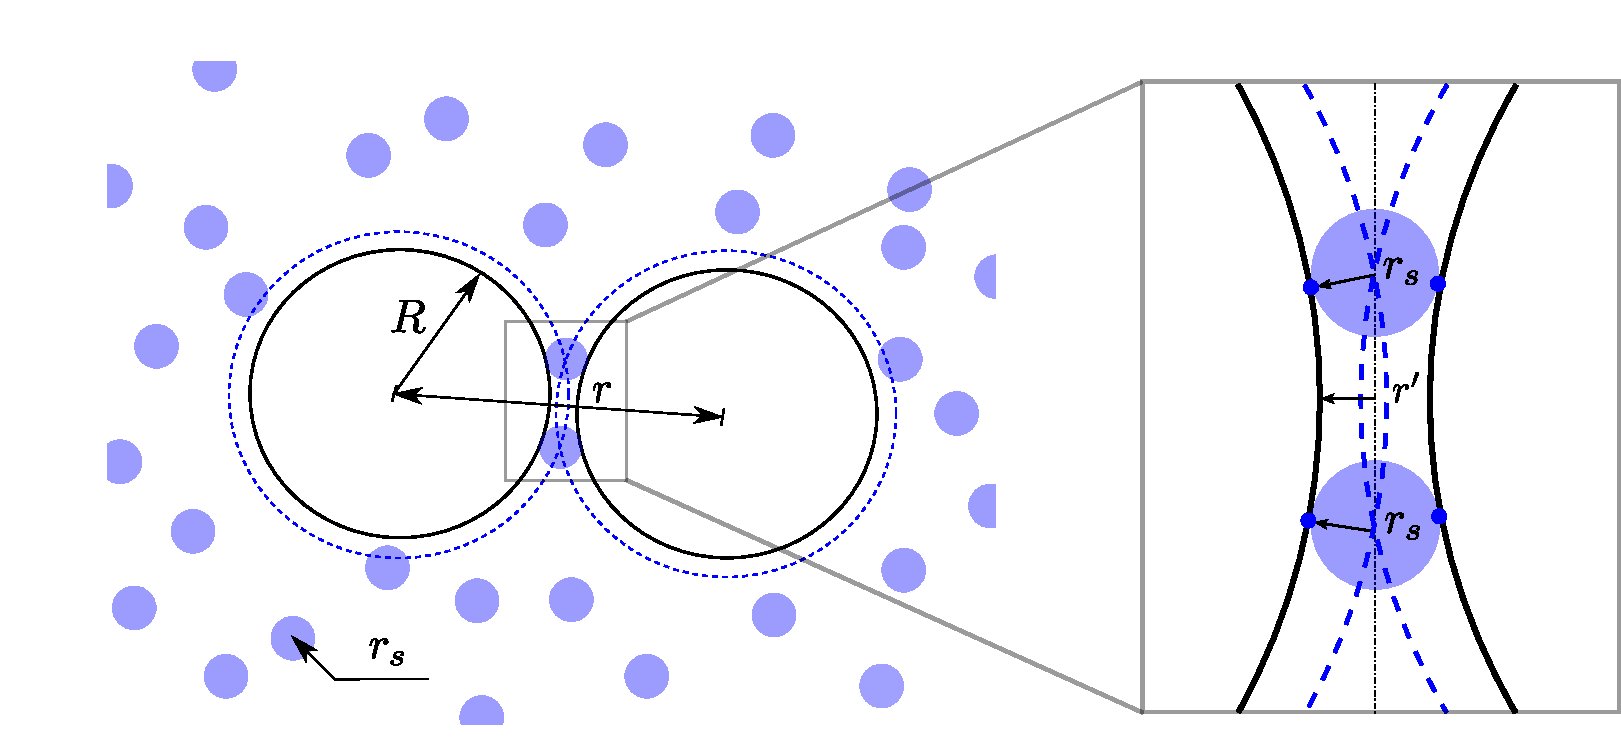
\includegraphics[width=7.2cm]{../paper1/Figures/depletion3.pdf}
  \end{textblock}
  
  \only<2-4>{
    \begin{textblock}{90}(3,50)
      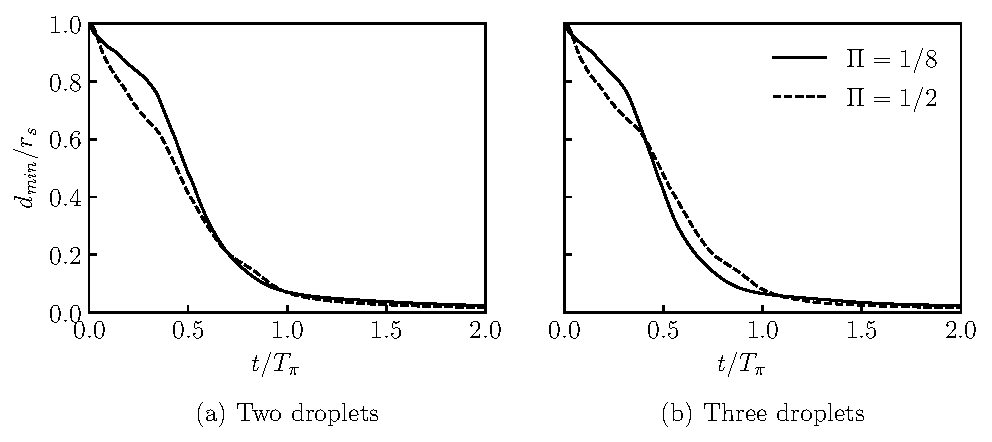
\includegraphics[width=\textwidth]{../paper2/figs/min_dist4.pdf}
    \end{textblock}
    \begin{textblock}{90}(33,63)
      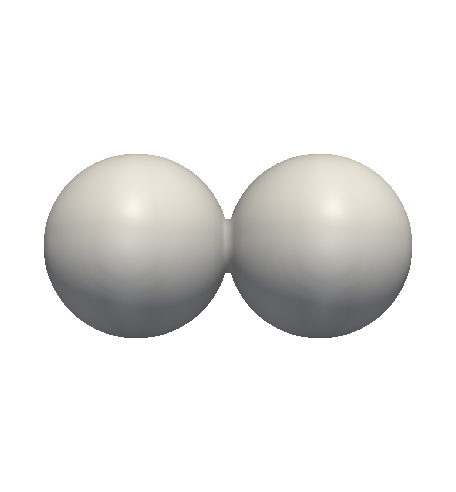
\includegraphics[height=1.1cm]{../paper2/figs/2dp.png}
    \end{textblock}
    \begin{textblock}{90}(76,63)
      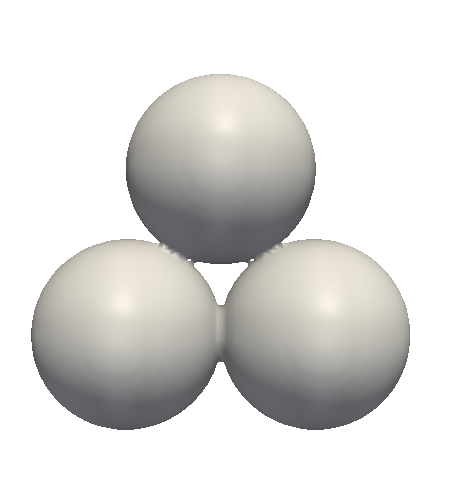
\includegraphics[height=1.1cm]{../paper2/figs/3dp.png}
    \end{textblock}
  } %end only

  \only<4->{
    \begin{textblock}{65}(93,50)
      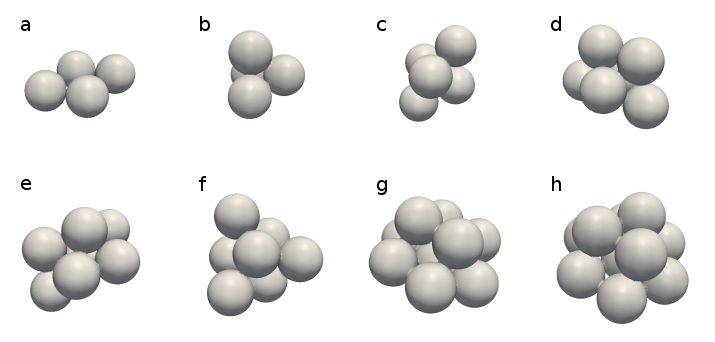
\includegraphics[width=\textwidth]{../paper2/figs/packings.png}
    \end{textblock}
  } %end only

  \only<5->{ 
    \begin{textblock}{90}(5,41)
      In summary, the depletion attraction
      \vskip0.1cm
      \begin{itemize}
      \item is local (activated at nearly touching);
      \item acts in the radial direction; 
      \item has a fast relaxation time.
      \end{itemize}
    \end{textblock}
  } % end only

  \only<6->{ 
    \begin{textblock}{65}(10,65)
      \begin{bluecolorbox}[Effects of depletion force]
        \begin{itemize}
        \item Keep nearby droplets in touch.
        \item Preserve the initial positions in the absence of noise. 
        \end{itemize}
      \end{bluecolorbox}
    \end{textblock}
  } % end only
    
\end{frame}

%%2
\begin{frame}[t]
  \frametitle{Flow-assisted assembly: Sticky droplets in shear-driven channel flows}

  \begin{textblock}{70}(5,15)
    The simplest example is the simple shear flow.
  \end{textblock}

  \begin{textblock}{70}(80,15)
    \includegraphics[width=\textwidth]{imgs/shear1.png}
  \end{textblock}

  \only<2->{
    \begin{textblock}{70}(5,20)
      A pair of particles in unbounded simple shear flow can have two types of trajectories%
      \footnote<.->[frame]{Batchelor \& Green, J. Fluid. Mech. 56, (2), 375-400. (1972).}: \vskip0.1cm
      \begin{itemize}
      \item open trajectory
      \item closed trajectory
      \end{itemize}
      \vskip0.1cm
      The dynamics are completely autonomous. 
    \end{textblock}

    \begin{textblock}{70}(80,47)
      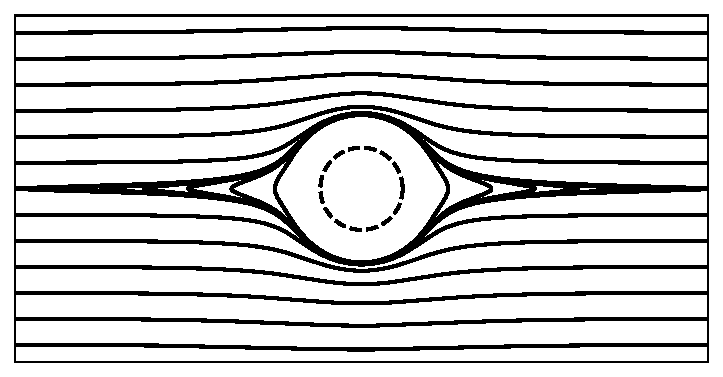
\includegraphics[width=\textwidth]{../imgs/BG-traj4.pdf}
    \end{textblock}
  } %end only

  \only<3->{
    \begin{textblock}{70}(5,50)
      Adding a depletion force shall not alter the phase portrait, since the force is local.%
      \footnote<.->[frame]{This is only true mathematically. Physically, there will be noise and the symmetry is not guaranteed.}
    \end{textblock}
  } %end only

  \only<4->{
    \begin{textblock}{70}(5,60)
      \xb{However, adding both depletion and confinement will profoundly change the droplet dynamics.}
    \end{textblock}
  } %end only
    
\end{frame}

%%2.0
\begin{frame}[t,noframenumbering]
  \frametitle{Flow-assisted assembly: Sticky droplets in shear-driven channel flows}

  \begin{textblock}{140}(5,15)
    To see that, we simulate a pair of touching droplets in a shear-driven channel of height $L_z=1.5D$. \vskip0.1cm
    \only<2->{
      Without the depletion attraction, droplets {\bf separate} and {\bf swap} their positions (i.e.\ symmetrical).%
      \footnote<.->[frame]{M. Zurita-Gotor \etal J. Fluid. Mech. 592, 447-469. (2007). I. Fouxon \etal ArXiv:1908.11208.}
    } %end only
    \only<3->{
      \vskip0.1cm
      With the depletion attraction and a strong confinement, only {\bf one configuration} is dynamically stable (i.e.\ the symmetry is lost).
    } %end only      
  \end{textblock}

  \only<1-2>{
    \begin{textblock}{105}(25,35)
      \movie[]{\includegraphics[width=\textwidth]{imgs/shear1.png}}
            {videos/shear-swap-no-depl.ogv}
    \end{textblock}
  } % end only

  \only<3-5>{
    \begin{textblock}{75}(7,35)
      \includegraphics[width=.3\columnwidth]{../paper2/figs/shear1.png}
      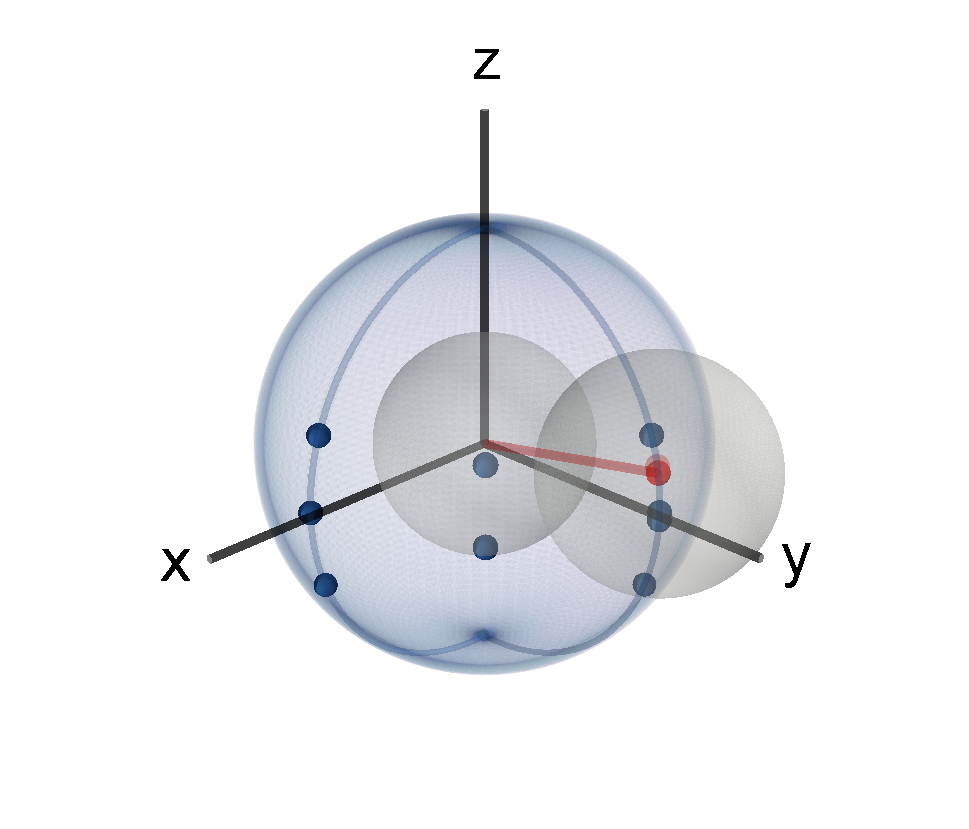
\includegraphics[width=.64\columnwidth]{../paper2/figs/shell1.png} 
    \end{textblock}
    \begin{textblock}{140}(12,80)
      Figure: All initial positions (\xb{blue dots}) stabalize at a polar angle $\theta_\infty=$ 79 deg (\xr{red dot}).
    \end{textblock}    
  } % end only
  
  \begin{textblock}{65}(80,45)
    \only<3>{
      \movie[]{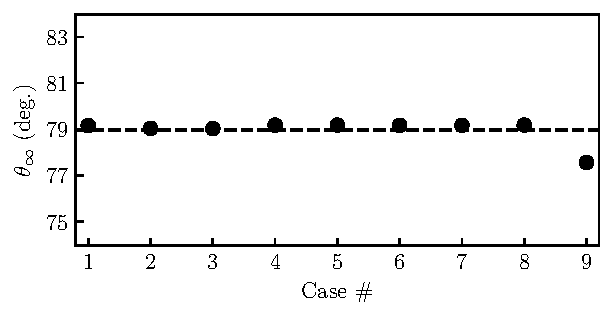
\includegraphics[width=.85\columnwidth]{../paper2/figs/angle_final2.pdf}}
            {videos/shear-align-case8.ogv}
    } %end only
    \only<4>{\includegraphics[width=\columnwidth]{imgs/traj0.pdf}}
    \only<5>{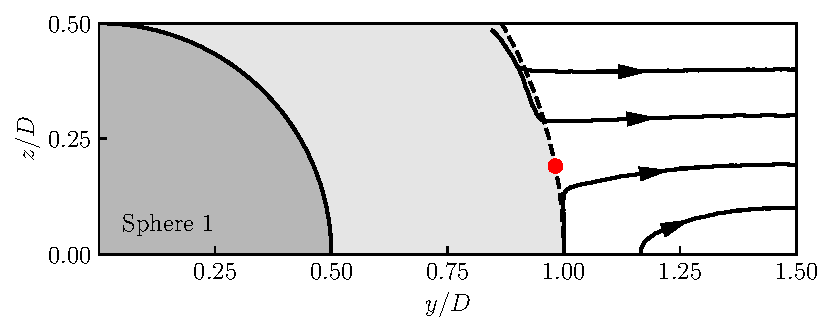
\includegraphics[width=\columnwidth]{imgs/traj.pdf}}
  \end{textblock}

  \only<6>{
    \begin{textblock}{92}(30,40)
        \begin{bluecolorbox}[Effects of depletion force $+$ shear $+$ confinement]
          \medskip
          \begin{itemize}
          \item It is a symmetry-breaking mechanism even at $N=2$. \medskip
          \item It leads to alignment in the flow direction. \medskip
          \item When $N>2$, we expect a chain of droplets. \medskip
          \end{itemize}
        \end{bluecolorbox}
      
    \end{textblock}
  } % end only

\end{frame}

%%
\begin{frame}[t]
  \frametitle{Flow-assisted assembly: Droplet clusters in pressure-driven channel flows}

  \begin{textblock}{145}(5,14)
    Finally, we turn to pressure-driven channel flows, the case that has the most resemblance to the actual microfluidic channel.
  \end{textblock}

  \begin{textblock}{80}(5,24)
    \only<2->{In the region far away from the inlet: homogeneous flow \vskip0.1cm
      \begin{itemize}
      \item w/o depletion force $\rightarrow $ {\bf scattering} drops
        \only<3->{
        \item w/ depletion force $\rightarrow$ forming a \only<3-4>{chain \only<4>{or a triangle}}\only<5->{{\bf chain} or a triangle}
        } %end only
      \end{itemize}
    } % end only
    
    \vskip0.1cm
    \only<6->{In the region close to the inlet:
      \begin{itemize}
      \item Non-uniform inflow \only<7->{$\rightarrow $ {\bf compact} clusters}
      \end{itemize}
    } % end only
    
  \end{textblock}

  \only<1-7>{
    \begin{textblock}{55}(12.5,49)
      \includegraphics{imgs/espci-chip-cartoon.png}
    \end{textblock}
  } %end only            
  
  \only<8>{
    \begin{textblock}{73}(5,52)
      \begin{bluecolorbox}[Effects of \emph{all} combined]
        \medskip
        \begin{itemize}
        \item Depletion force is necessary for cluster formation. %\medskip
        \item Confined homogeneous shear flow promotes droplet chains. %\medskip
        \item Non-uniform inflow can lead to compact structures (with some tuning). %\medskip
        \item Overall, these are 3D effects. \medskip
        \end{itemize}
      \end{bluecolorbox}
    \end{textblock}
  } % end only

    \begin{textblock}{67}(85,30)
      \begin{figure}
      %\centering
      \only<2>{
        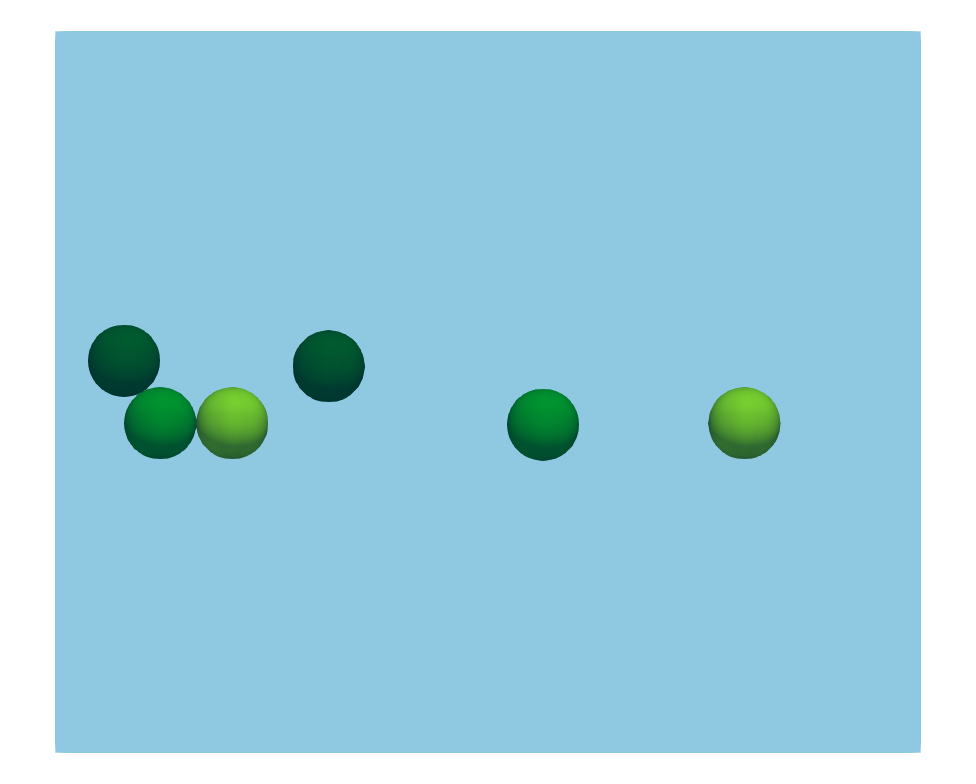
\includegraphics[width=.7\columnwidth]{../paper2/figs/3-scatter-top.png}
        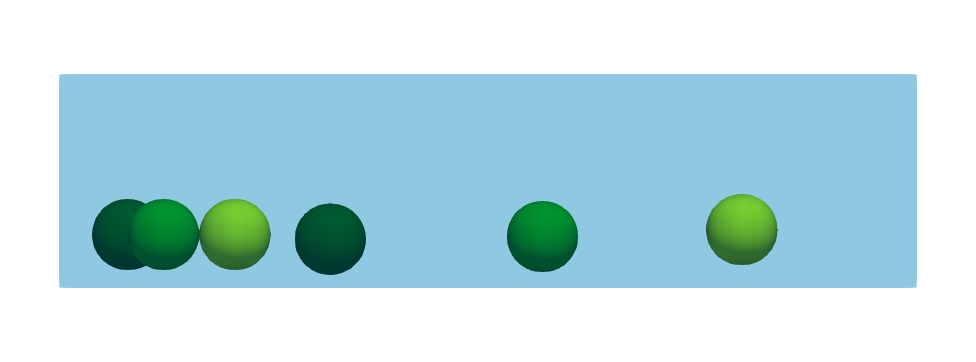
\includegraphics[width=.7\columnwidth]{../paper2/figs/3-scatter-side.png}
        \vskip0.2cm \hskip0.4cm
        %Without depletion force: scattering drops.
      } % end only
      \only<3>{
        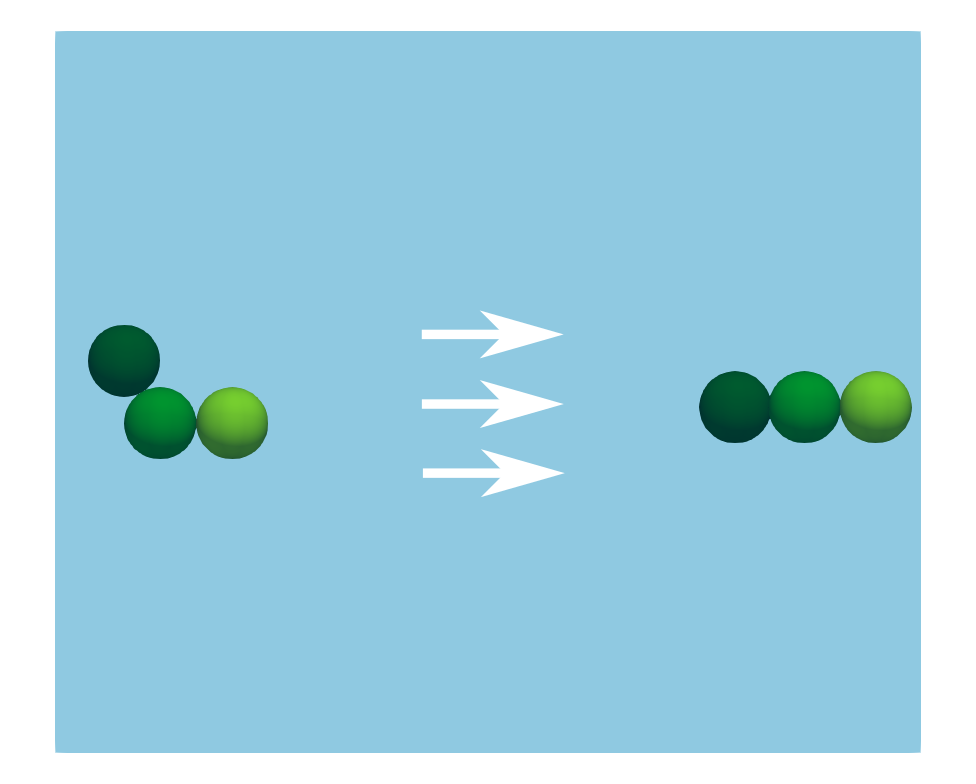
\includegraphics[width=.7\columnwidth]{../paper2/figs/3-line-top1.png}
        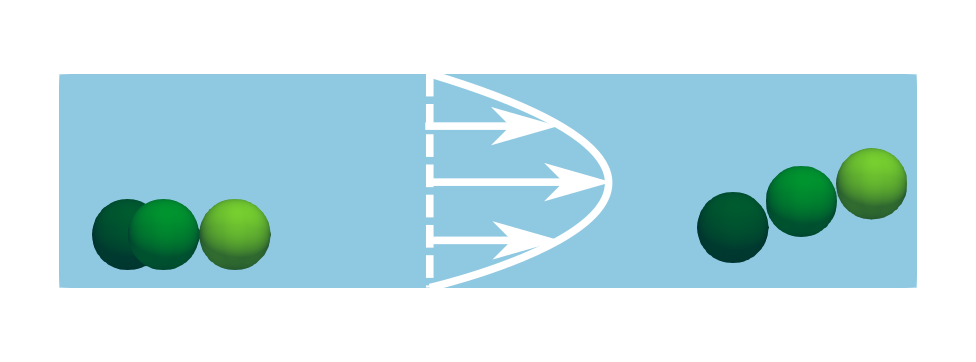
\includegraphics[width=.7\columnwidth]{../paper2/figs/3-line-side1.png}
        \vskip0.2cm \hskip0.4cm
        %With depletion force: forming a chain.
      } % end only
      \only<4>{
        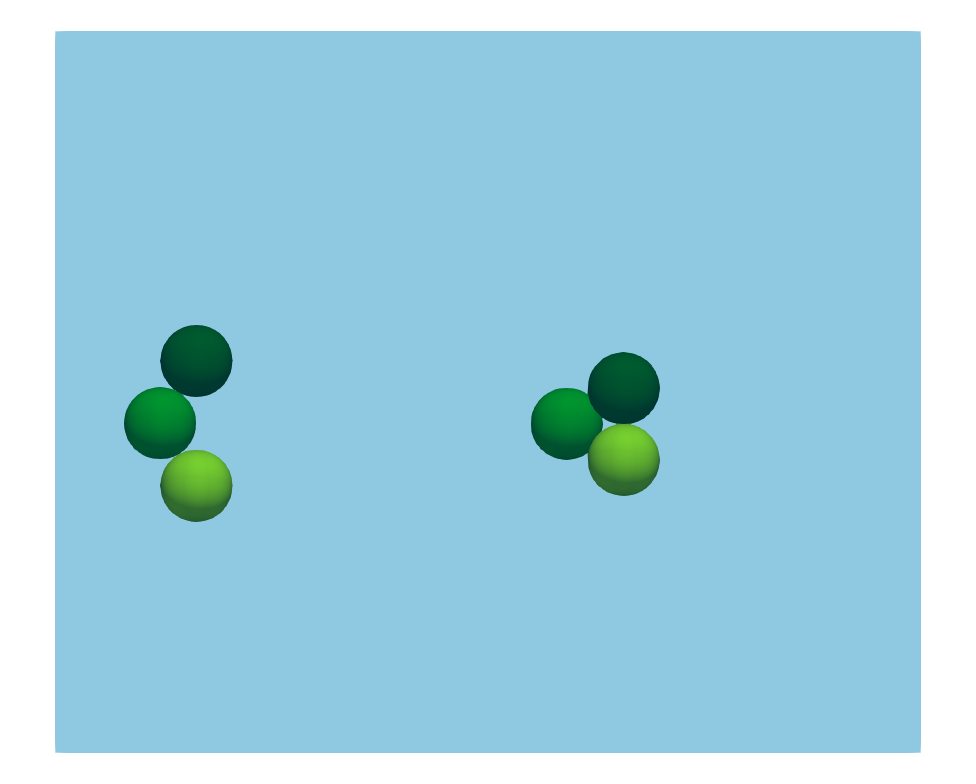
\includegraphics[width=.7\columnwidth]{../paper2/figs/3-triangle-top.png}
        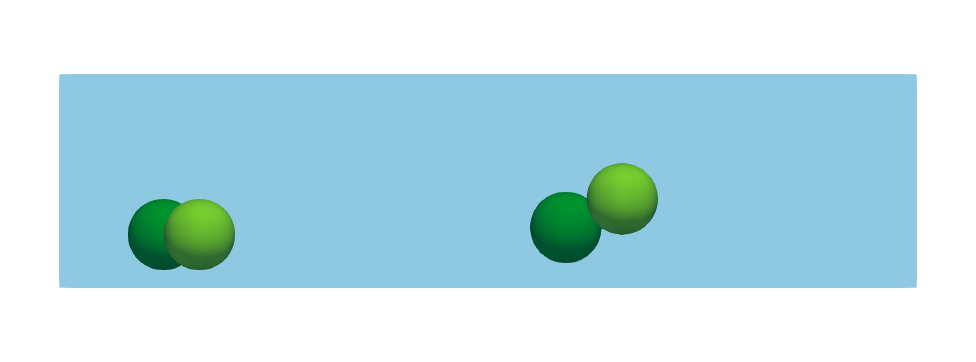
\includegraphics[width=.7\columnwidth]{../paper2/figs/3-triangle-side.png}
        \vskip0.2cm \hskip0.4cm
        %With depletion force: forming a triangle.
      } % end only
      \only<5>{
        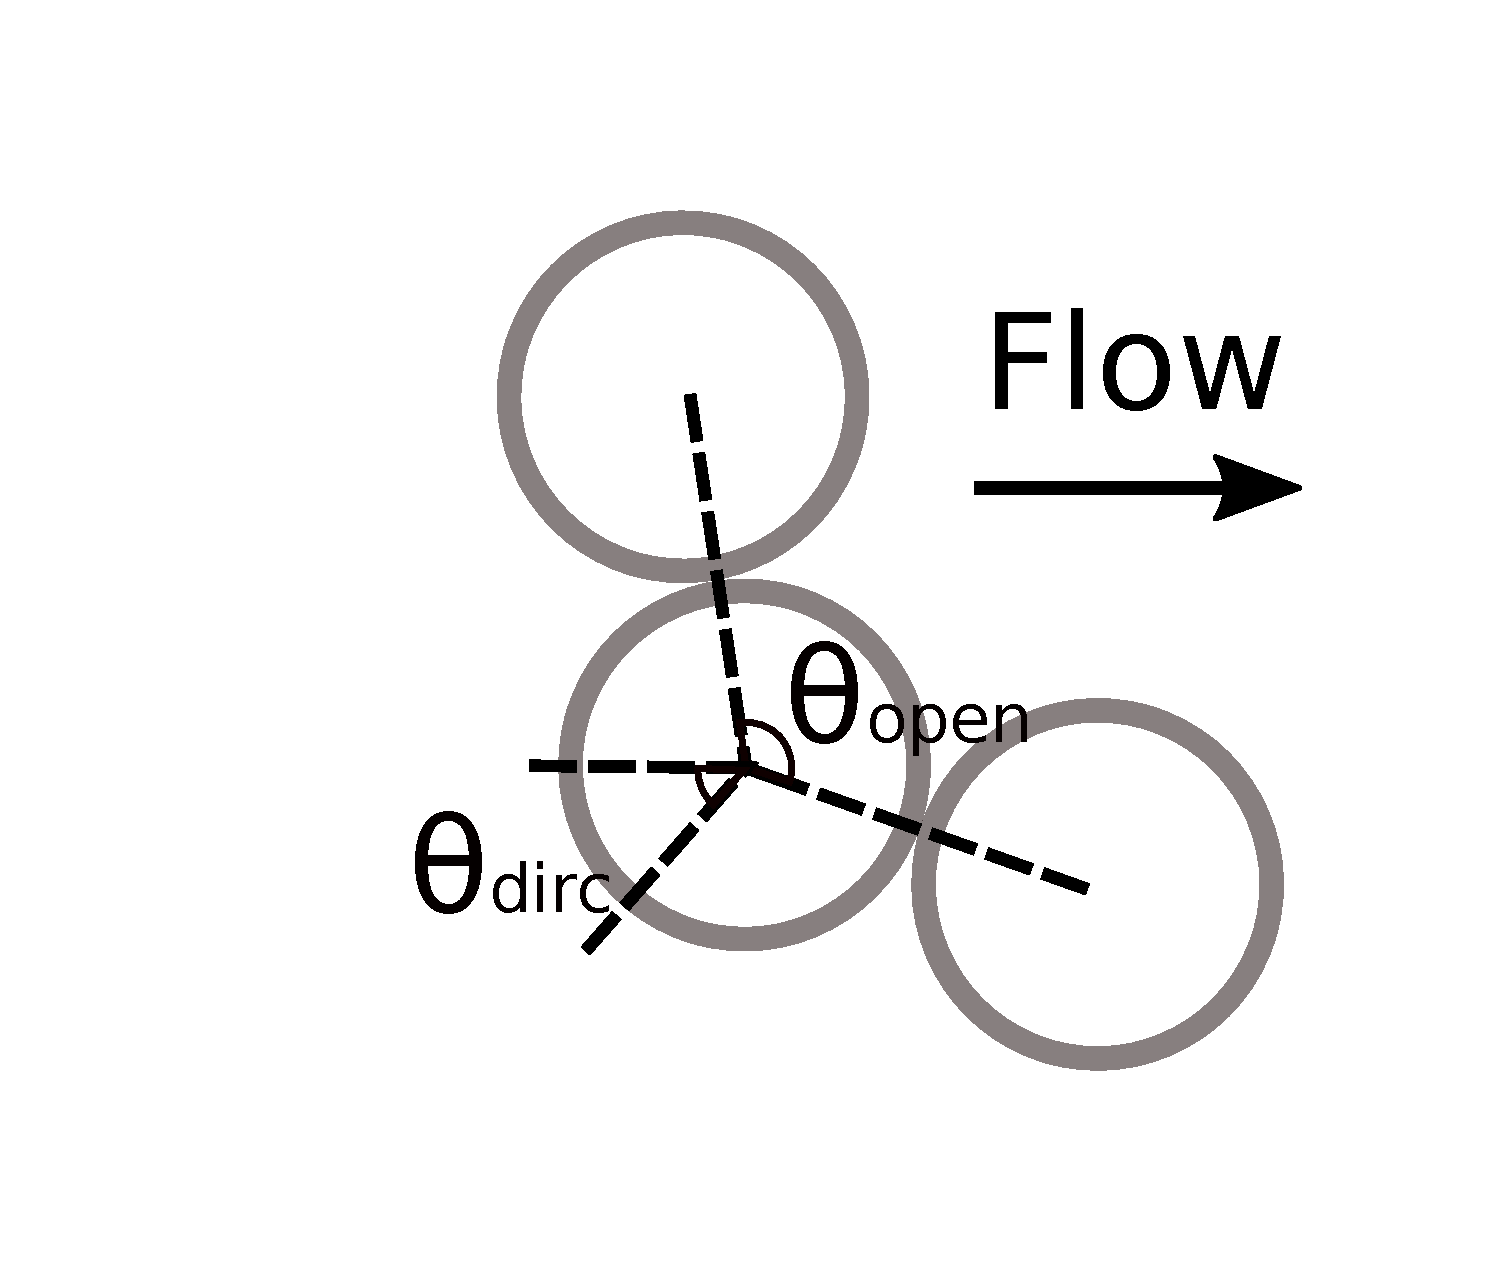
\includegraphics[width=.5\columnwidth]{../paper2/figs/angle_sketch1.pdf}
        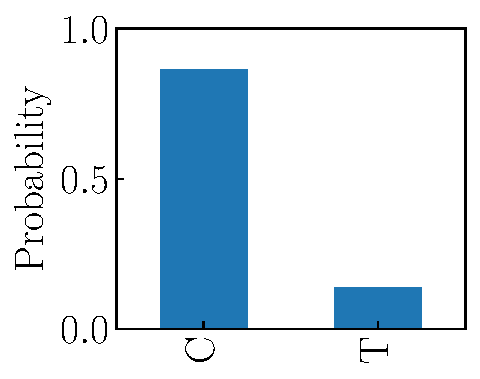
\includegraphics[width=.5\columnwidth]{../paper2/figs/result_poi_bar.pdf}
        \vskip0.2cm \hskip0.2cm
        Overall, chains are more favorable than triangles.
      } % end only
      \only<6>{
        \vskip1cm
        \movie[]{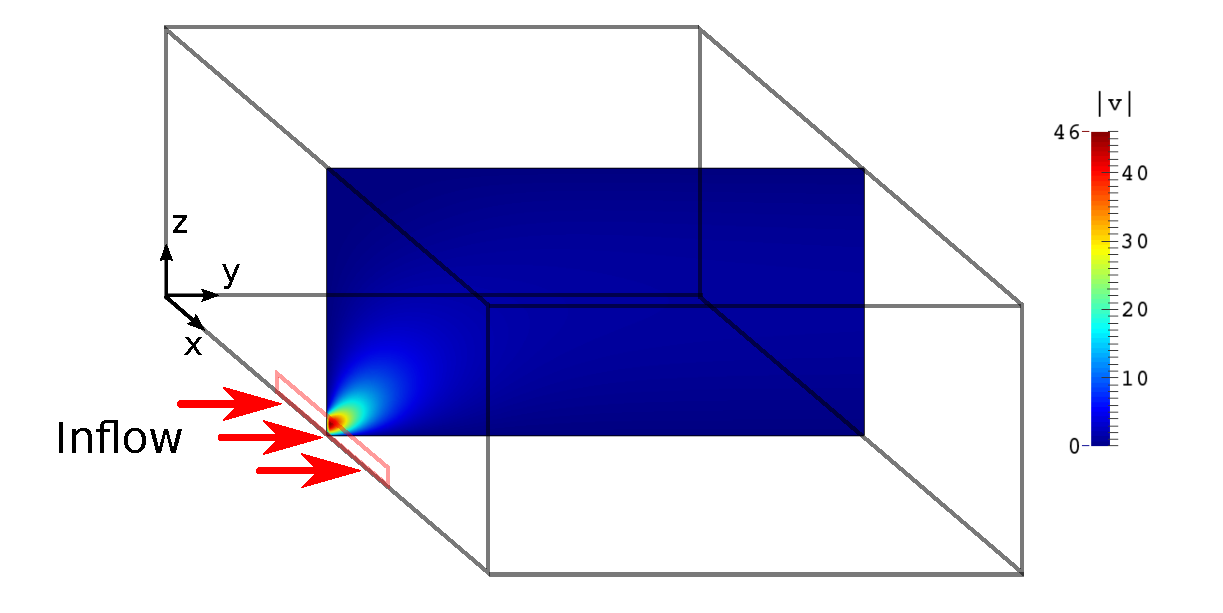
\includegraphics[width=\columnwidth]{../paper2/figs/non-uniform_inflow1.pdf}}
              {videos/movie-bird.ogv}
        \vskip0.2cm \hskip0.2cm
        %A very non-uniform inflow.
      } % end only
      \only<7-8>{
        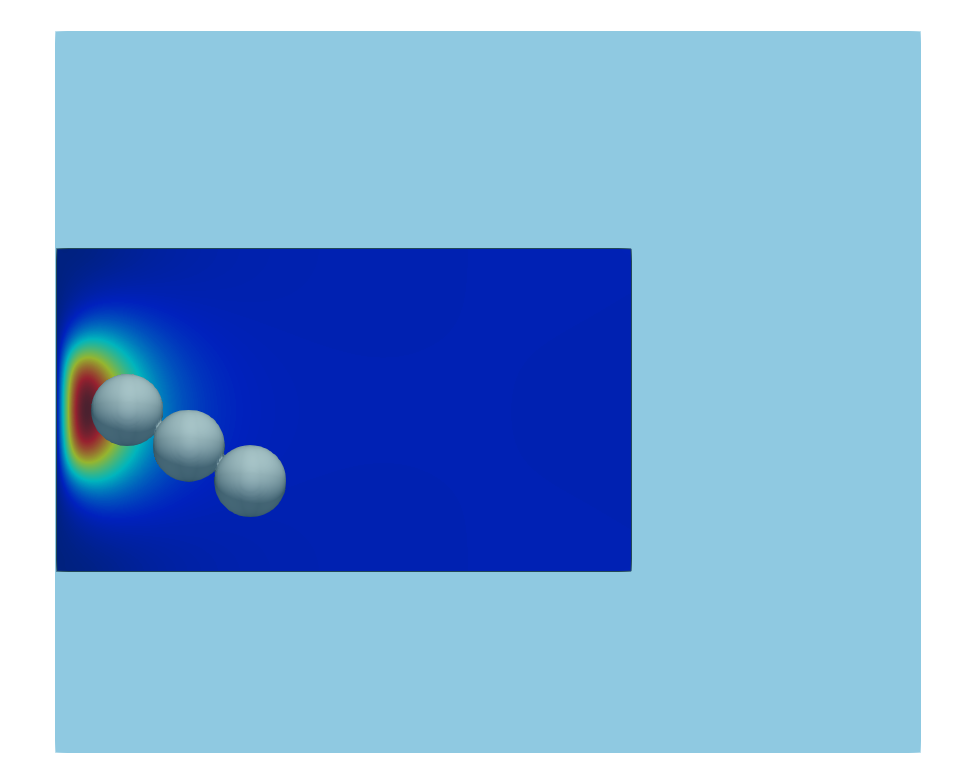
\includegraphics[width=.32\columnwidth]{../paper2/figs/bx6-top-0.png}
        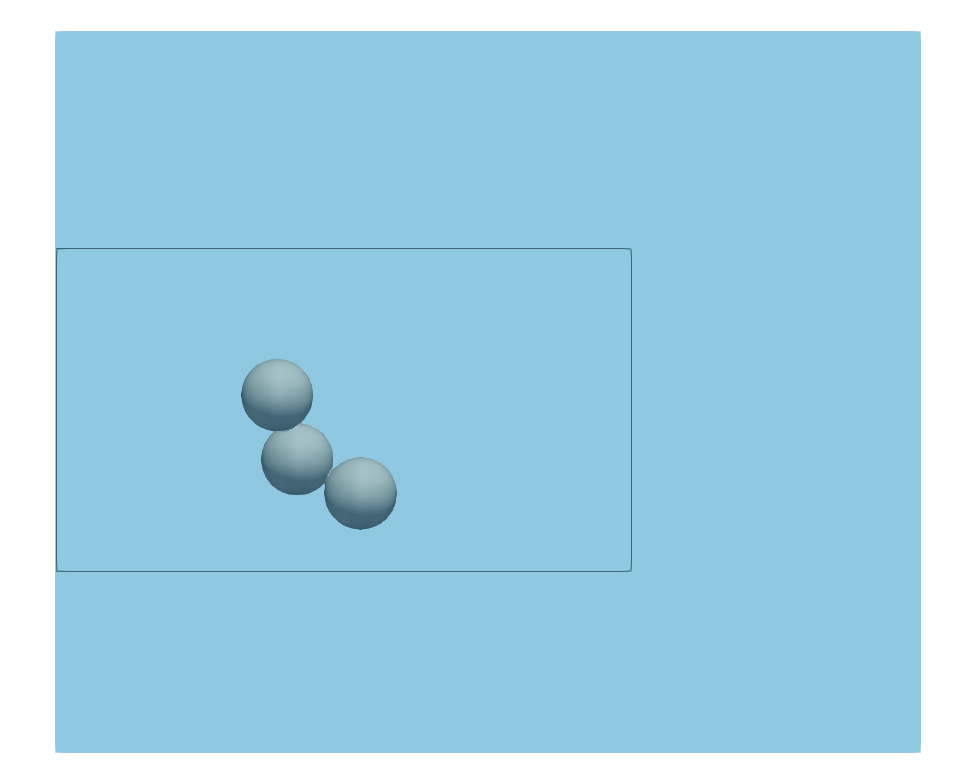
\includegraphics[width=.32\columnwidth]{../paper2/figs/bx6-top-150k-l.png}
        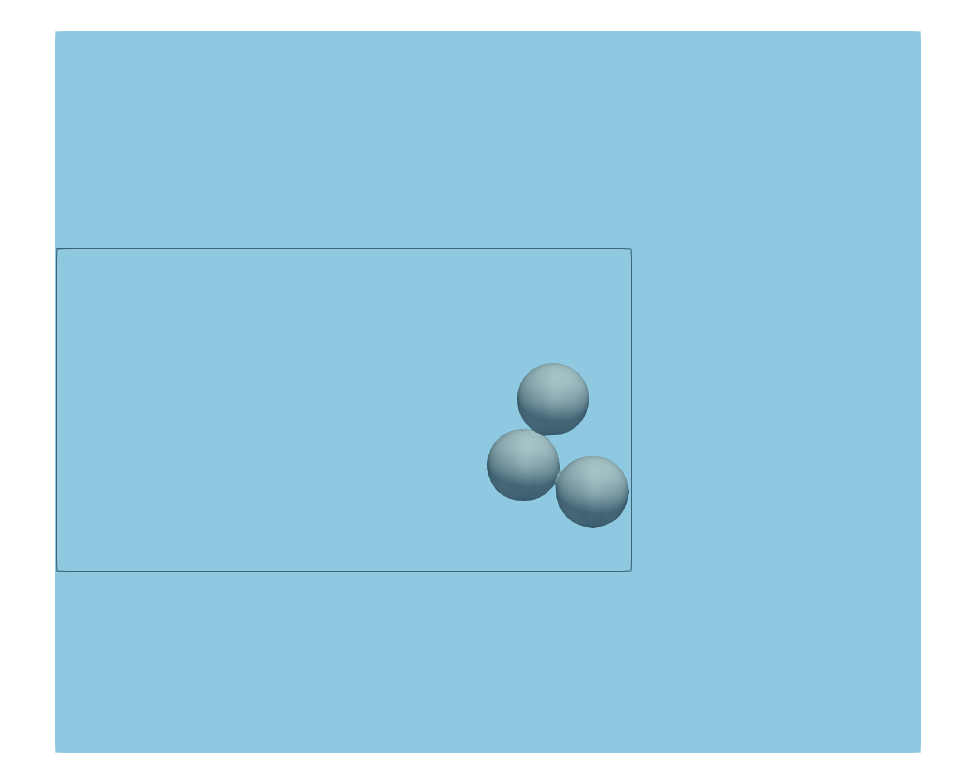
\includegraphics[width=.32\columnwidth]{../paper2/figs/bx6-top-570k.png}
        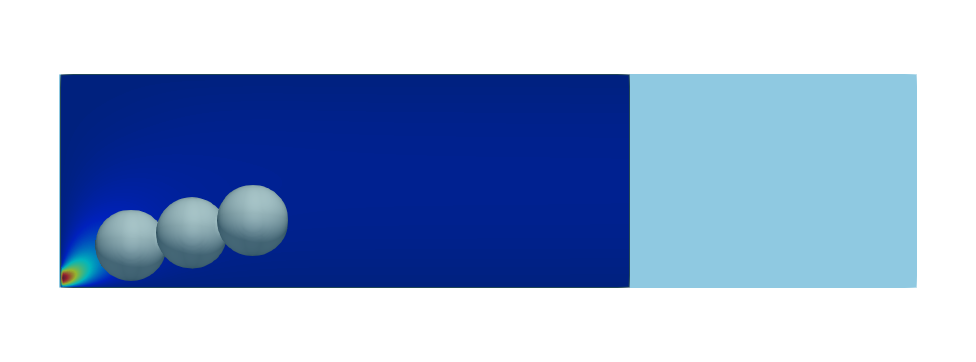
\includegraphics[width=.32\columnwidth]{../paper2/figs/bx6-side-0.png}
        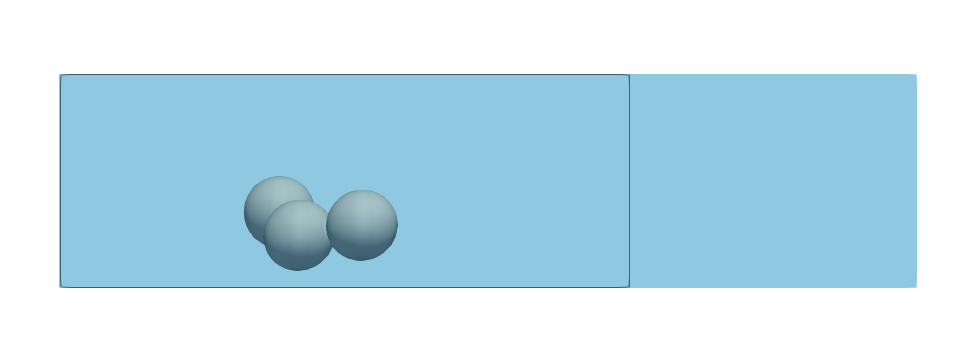
\includegraphics[width=.32\columnwidth]{../paper2/figs/bx6-side-150k-l.png}
        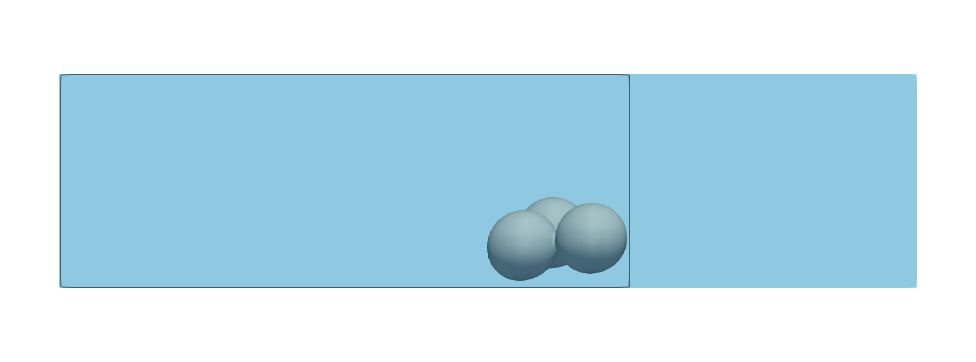
\includegraphics[width=.32\columnwidth]{../paper2/figs/bx6-side-570k.png} 
        
\includegraphics[width=.75\columnwidth]{../paper2/figs/time_arrow.pdf}
        \includegraphics[width=.32\columnwidth]{../paper2/figs/bd8-top-0.png}
        \includegraphics[width=.32\columnwidth]{../paper2/figs/bd8-top-150k.png}
        \includegraphics[width=.32\columnwidth]{../paper2/figs/bd8-top-450k.png}
        \includegraphics[width=.32\columnwidth]{../paper2/figs/bd8-side-0.png}
        \includegraphics[width=.32\columnwidth]{../paper2/figs/bd8-side-150k.png}
        \includegraphics[width=.32\columnwidth]{../paper2/figs/bd8-side-450k.png}
        \vskip0.2cm \hskip0.2cm
        Assembly of 3-4 droplets.
      } % end only
      \end{figure}
    \end{textblock}
    
  
  
\end{frame}

%%
\begin{frame}[t]
  \frametitle{Flow-assisted assembly: But what about the dipolar interactions?}

  \begin{columns}[T]
    
    \begin{column}{0.45\textwidth}
      \centering
      \only<1>{
        \includegraphics[height=4cm]{imgs/espci-chip-cartoon.png}
        \includegraphics[height=2.8cm]{imgs/espci-dipolar-cartoon.png}
      } % end only
      \only<2->{
        \begin{figure}
          \includegraphics[width=\columnwidth]{../paper3/flow_vort-40k_small.pdf}
          \caption{Depth-averaged disturbance flow around a sphere travelling in the $x'$ direction.
            The particle is located in the middle of a pressure-driven channel with $H/D=1.5$.%
            \footnote<2->[frame]{Fouxon \etal Phys. Rev. E. 96, 063110 (2017).}}
        \end{figure}
      } %end only
    \end{column}

    \begin{column}{0.45\textwidth}
      
      \begin{bluecolorbox}[Hypotheses]
        \begin{itemize}
        \item Droplets obey laws in quasi-two- dimensional (q2D) space.
        \item Depletion force attracts nearby drops.
        \item Hydrodynamic interactions (HI) lead to the rearrangement dynamics.
        \end{itemize}
      \end{bluecolorbox}

      \vskip.3cm
      \begin{bluecolorbox}[Equations of motion (due to HI)]
        \begin{equation} \notag
          \begin{aligned}
            & {\bm u}^\infty(x,y,z) \approx -\frac{z(H-z)}{2\mu} \nabla p(x,y), \\
            & \delta{\bm u}_{ij} = {\bm B}_{ij} {\bm F}_j, \quad {\bm U}_i = {\bm u}^\infty_i + \sum_{j \ne i} \delta{\bm u}_{ij},
          \end{aligned}
        \end{equation}
        where
        \begin{equation} \notag
          \begin{aligned}
            {\bm B}({\bm x}) \approx -\frac{\alpha H}{\mu} \bigg( \frac{{\bm I}}{\abs{\bm x}^2} -
            \frac{ 2{\bm x}{\bm x} }{ \abs{{\bm x}}^4} \bigg).
          \end{aligned}
        \end{equation}
      \end{bluecolorbox}
    \end{column}

  \end{columns}

  \only<3->{
    \begin{textblock}{80}(91,92)
      \xb{However, the prefactor is $\sim \mathcal{O}(10^{-2})$.}
    \end{textblock}
  } % end only
  
  \only<4->{
    \begin{textblock}{100}(8,87)
      \xr{\bf The picture is correct; but the number is wrong.}
    \end{textblock}
  }% end only
  
\end{frame}

%%
\hypertarget{conclusion1}{%
  \subsection{Conclusions}}

\begin{frame}[t]
  \frametitle{Conclusions}

  \vskip0.1cm
  \begin{columns}[T]
    
    \begin{column}{0.95\textwidth}
      \begin{bluecolorbox}[Droplet interactions]
        %\medskip
        \begin{itemize}
        \item Droplets in confined 3D geometries, such as the one we considered here, do obey laws in q2D (e.g.\ dipolar interactions).
          \only<2->{However, the interaction is too weak to produce the dynamics observed within the time scale of the experiment.}
          \only<3->{Therefore, it can only be used as a \emph{far-field} approximation in the \emph{long-time} limit.}
          \only<4->{\medskip 
          \item The correct explanation for the experimental observation is based on a number of 3D effects,
            such as the confinement-mediated shear alignment, inhomogeneous boundary conditions, \emph{etc}.}
          \only<5->{However, the interplay of these 3D effects negates a simple droplet interaction model of parametric dependence.}
          \only<6->{In practice, we may have to do a \emph{full} simulation for each setup to predict the droplet dynamics,
            and it remains difficult to make a diamond cubic. }
        \end{itemize}
      \end{bluecolorbox}

      \vskip0.3cm
      \only<7->{
        \begin{bluecolorbox}[Photonic material fabrication]
          %\medskip
          \begin{itemize}
          \item It's still possible to make PhC using the microfluidic-based approach,
            e.g.\ an ingeneous approach has been proposed to assemble face-centered cubic composed of smaller clusters.%
            \footnote<.->[frame]{Morozov \& Leshansky, Langmuir. 35, 11, 3987-3991 (2019).}
            \only<8->{\medskip 
            \item However, instead of struggling with crystal making, the current fashion is to make \emph{disordered} photonic materials.%
              \footnote<.->[frame]{Ricouvier \etal PNAS. 116 (19), 9202-9207 (2019).}    }
          \end{itemize}
        \end{bluecolorbox}
      } %end only
    \end{column}
    
  \end{columns}
  
\end{frame}
%%2
\begin{frame}[noframenumbering,t]
  \frametitle{Conclusions}

  All the conclusions are based on the following papers.
  
  \begin{textblock}{45}(5,20)
    \begin{tcolorbox}[beamer,
        width=\textwidth,
        arc=0pt,
        boxsep=1pt,
        left=0pt,right=0pt,top=0pt,bottom=0pt,
      ]
      \includegraphics[width=\linewidth]{imgs/PRE_cover.png}
    \end{tcolorbox}
    Fouxon \etal PRE (2017).
  \end{textblock}

  \begin{textblock}{45}(55,20)
    \begin{tcolorbox}[beamer,
        width=\textwidth,
        arc=0pt,
        boxsep=1pt,
        left=0pt,right=0pt,top=0pt,bottom=0pt,
      ]
      \includegraphics[width=\linewidth]{imgs/soft-mat.png}
    \end{tcolorbox}
    Ge \etal Soft Matter (2019).
  \end{textblock}

  \begin{textblock}{45}(105,20)
    \begin{tcolorbox}[beamer,
        width=\textwidth,
        arc=0pt,
        boxsep=1pt,
        left=0pt,right=0pt,top=0pt,bottom=0pt,
      ]
      \includegraphics[width=\linewidth]{imgs/arxiv-cover.png}
    \end{tcolorbox}
    Fouxon \etal Under review.
  \end{textblock}

\end{frame}

%%
\hypertarget{part2}{%
  \section{Part II: Modelling Dense Suspensions (DS)}}

%%
\hypertarget{background2}{%
  \subsection{Soft matter and rheology}}

\begin{frame}[t]
  \frametitle{Soft matter and rheology}
  
  \begin{columns}[T]
    
    \begin{column}{0.65\textwidth}
      In his Nobel lecture (1991), de Gennes described two main features of \emph{soft matter}:
      \only<2->{
        \begin{itemize}
        \item complexity (he used the analogy of biology);
          \only<3->{\item flexibility (he used the example of rubber).}
        \end{itemize}
      } %end only
      \vskip0.2cm
      \only<4->{Specifically, groups of cells, proteins, polymers, surfactants, colloidal grains, {\it etc.} are all examples of soft matter.}
      \vskip0.2cm
      \only<5->{A better understanding of these systems \xb{in} and \xr{out of} equilibrium thus has many practical relevance.}
      \vskip0.2cm
      \only<6->{In particular, a currently active research area is {\bf dense suspension} (DS),
        where suspending particles occupy equal or more volume than the underlying fluid and
        interact strongly via short-range lubrication or non-hydrodynamic forces.}
      \vskip0.2cm
      \only<7->{This is intimately related to \emph{rheology}, the study of the deformation and flow of matter (in the overdamped regime).}
      \vskip0.2cm
      \only<8->{There are rich phenomena in DS, such as {\it shear thickening} or {\it jamming}.}
      \vskip0.2cm
      \only<9->{Questions regarding how such rheological behaviours depend on \xb{microscopic interactions}
        or \xb{particle/manifold geometries} are still not fully understood today.}
    \end{column}

    \begin{column}{0.25\textwidth}      
      %\vskip.5cm
      \begin{figure}
        \centering
        \only<2->{
          \includegraphics[width=\columnwidth]{imgs/ecoli.jpg}
          \caption{E. coli.}
        } % end only
        \vskip0.1cm
        \only<6->{
          \includegraphics[width=\columnwidth]{../paper7/figs/np2000_vol0.55.png}
          \caption{$N=2000$, $\phi=55$\%.}
        } % end only
      \end{figure}
    \end{column}
  \end{columns}

\end{frame}

%%
\hypertarget{simulation2}{%
  \subsection{Numerical modelling}}

\begin{frame}[t]
  \frametitle{Numerical modelling -- Why?}

  \begin{textblock}{129}(5,14)
  For DS far from equilibrium, there is no established analytical method to study the system behaviour bottom-up.
  \vskip0.2cm
  \only<2->{The difficulty is mainly mathematical (a case of the \xr{$N$-body problem}).}
  \vskip0.2cm
  \only<3->{On the other hand, solving a system of interacting particles is relatively straightforward in an \xb{algorithmic} perspective.}
  \vskip0.2cm
  \only<4->{That is, we can use computers to solve the $N$-body dynamics in a brute-force manner.}
  \vskip0.2cm
  \only<5->{Furthermore, in the DS context, numerical simulations have demonstrated a unique capability to%
    \footnote<.->[frame]{E. Del Gado \& J. Morris. J. Rheol. 64, 223 (2020).} \vskip0.1cm
    \only<6->{\begin{itemize}
      \item provide insight into microscopic mechanisms;\vskip0.1cm
      \only<7->{\item abstract the fundamental underpinnings of the rheological response;\vskip0.1cm}
      \only<8->{\item help one to link experiments and theory in a consistent picture.}
      \end{itemize}
    } %end only
  } %end only
  \vskip0.2cm
  \only<9->{\xb{\bf Therefore, we aim to develop and implement a numerical model to study DS.}}
  \end{textblock}
    
\end{frame}

%%
\hypertarget{hlgd}{%
  \subsubsection{HLGD}}

\begin{frame}[t]
  \frametitle{Numerical modelling -- How?}

  \begin{columns}[T]

    \begin{column}{0.4\textwidth}
      \vskip0.2cm
      There are at least four classes of methods to simulate DS (in increasing efficiency):
      \vskip0.2cm
      \only<2->{
        \begin{itemize}
        \item Finite volume solvers \vskip0.2cm
        \only<5->{\item Boundary integral methods \vskip0.2cm}
        \only<7->{\item Stokesian dynamics (SD) \vskip0.2cm}
        \only<13->{\item Hybrid lubrication/granular dynamics (HLGD).}
        \end{itemize}
      } % end only

      \vskip0.4cm
      \only<14->{
        \xb{\bf We implemented a version of HLGD to study DS.}%
        \footnote<.->[frame]{Lees-Edwards boundary condition, velocity-Verlet integration, near-neighbour list, {\it etc.}}
      } % end only
    \end{column}
    
    \begin{column}{0.56\textwidth}
      \only<2->{
        \vskip-0.1cm
        \begin{bluecolorbox}[Mathematical formulation]
          \only<2-4>{
            The incompressible Navier-Stokes (NS) equations read,
            \begin{subequations} 
              \begin{equation}\tag{1a}
                \nabla \cdot {\bm u} = 0,
                \label{eq:div-free}
              \end{equation}
              \begin{equation} \tag{1b}
                \rho \bigg(\frac{\partial {\bm u}}{\partial t} + {\bm u} \cdot \nabla {\bm u} \bigg) = \nabla \cdot {\bm \sigma} + {\bm f},
                \label{eq:NS}
              \end{equation}
            \end{subequations}
            where $\bm \sigma$ is the viscous stress tensor, given as
            \begin{equation} \tag{2}
              \begin{aligned}
                {\bm \sigma} = -p {\bm I}+ \mu \bigg( \nabla {\bm u} + (\nabla {\bm u})^T \bigg),
              \end{aligned}
            \end{equation}
            and is subject to the following boundary condition across the interface
            \begin{equation} \tag{3}
              ({\bm \sigma}_+ - {\bm \sigma}_- ) \cdot {\bm n} = \gamma \kappa {\bm n} - \nabla \gamma.
            \end{equation}
            \vskip0.2cm
            
            \only<3-4>{
              In the case of Stokes flow, Eq.\ \eqref{eq:NS} becomes,
              \begin{equation} \notag
                \nabla \cdot {\bm \sigma} + {\bm f} =0.
              \end{equation}
              \vskip0.1cm
              \only<4>{In any case, the \emph{whole domain} needs to be meshed.}
            } % end only
          } %end only
          
          \only<5-6>{
            An integral representation of the velocity field in Stokes flow,
            \begin{equation} \notag
              \begin{aligned}
                u_i(\bm{x}) - u_i^\infty(\bm{x}) = -\frac{1}{8\pi \mu} \sum_{\alpha=1}^N  \int_{S_\alpha} G_{i,j} (\bm{x},\bm{x}_0) f_j(\bm{x}_0) dS_{x_0},
              \end{aligned}
            \end{equation}
            where $\bm{u}^\infty(\bm{x})$ is the velocity at position $\bm{x}$ in the absence of particles,
            $S_\alpha$ is the surface of particle $\alpha$,
            $\bm{G}(\bm{x},\bm{x}_0)$ is the Stokeslet due to a point force at $\bm{x}_0$,
            $\bm f(\bm{x}_0)$ denotes its density,
            and the summation is over all $N$ particles. \vskip0.2cm
            \only<6>{
              The integral on the r.h.s of the equation can be evaluated numerically by meshing the \emph{particle surface}.
            } % end only
          } % end only
          
          \only<7-8>{
            SD rewrites the integral as a multipole expansion,
            \begin{equation} \notag
              \begin{aligned}
                - \frac{1}{8\pi \mu} \sum_{\alpha=1}^N  \int_{S_\alpha} ... \approx \bm{u}_F + \bm{u}_S + \bm{u}_T + \bm{u}_Q + \bm{u}_O , 
              \end{aligned}
            \end{equation}
            where $\bm{u}$'s denote the flow due to leading-order poles. \vskip0.1cm
            \only<8>{
              The multipole expansion can then be combined with the Fax\'{e}n's formulae for spheres
              to obtain a relationship between particle velocities and forces,
              \begin{equation} \notag
                \begin{aligned} 
                  \begin{pmatrix}
                    {\bm U}-{\bm U}^\infty \\
                    -{\bm E}^\infty
                  \end{pmatrix}
                  = \mathscr{M^\infty} \cdot
                  \begin{pmatrix}
                    {\bm F}^H \\
                    {\bm S}^H
                  \end{pmatrix},
                \end{aligned}
              \end{equation}
              where $\mathscr{M}^\infty$ is the far-field ``grand mobility'' matrix. \vskip0.1cm
            } % end only
          } % end only

          \only<9-10>{
            The grand mobility matrix may be inverted to obtain the ``grand resistance'' matrix $\mathscr{R}$, 
            \begin{equation} \notag
              \begin{aligned} 
                \begin{pmatrix}
                  {\bm F}^H \\
                  {\bm S}^H
                \end{pmatrix}
                = \mathscr{R} \cdot
                \begin{pmatrix}
                  {\bm U}-{\bm U}^\infty \\
                  -{\bm E}^\infty
                \end{pmatrix},
              \end{aligned}
            \end{equation}
            which, once obtained, can be used to calculate $\bm U$. \vskip0.1cm
            \only<10>{
              Overall, the dynamics is governed by
              \begin{equation} 
                \begin{aligned} \notag
                  {\bm m} \cdot \frac{d{\bm U}}{dt} = {\bm F}^H + {\bm F}^A,
                \end{aligned}
              \end{equation}
              which can be solved \emph{without meshing anything}.
            } % end only
          } %end only

          \only<11->{
            In SD, lubrication is explicitly accounted for in $\mathscr{R}$,
            \begin{equation} \notag
              \begin{aligned}
                \mathscr{R} = (\mathscr{M}^\infty)^{-1} +\mathscr{R}_{2B} - \mathscr{R}_{2B}^\infty,
              \end{aligned}
            \end{equation}
            where $\mathscr{R}_{2B}^\infty$ denotes the duplication terms. \vskip0.1cm
            \only<12->{ 
              Since lubrication diverges at contact, which is more probable at higher concentrations,
              we can further simplify $\mathscr{R}$ as,
              \begin{equation}  \notag
                \begin{aligned}
                  \mathscr{R} = \mathscr{R}_{2B}.
                \end{aligned}
              \end{equation}
            } %end only
            \only<13->{
              \vskip.01cm
              This, combined with models for contact forces (e.g.\ collision and fricition), is the mathematical basis of HLGD.
            } %end only
          } %end only
          
        \end{bluecolorbox}

        %\only<11->{
        %  \vskip0.4cm
        %  \centering
        %  \includegraphics[width=0.85\columnwidth]{../imgs/stick-slide.pdf}
        %} % end only
      } %end only
    \end{column}
    
  \end{columns}
  
\end{frame}

%%
\hypertarget{Cases}{%
  \subsection{Case studies}}
%%1
\begin{frame}[t]
  \frametitle{Case studies -- Jamming transition}
  
  We simulate 200 spherical particles, initially randomly distributed in a cubic box, undergoing simple shear. \vskip0.1cm
  \only<2->{
    The particles experience Stokes drag, lubrication, and collision forces. \vskip0.1cm}
  \only<3->{
  We plot the relative viscosity, $\eta_r=\sigma_{xy}/(\mu\dot{\gamma})$,
  and non-dimensional particle pressure, $\eta_n=-\textrm{tr}(\bm{\sigma})/(3\mu\dot{\gamma})$, as functions of volumn fraction.
  \vskip0.2cm}

  \only<1-3>{
    \begin{textblock}{110}(52,40)
      \includegraphics[width=0.47\textwidth]{imgs/suspension-shear.png}\\
      {\footnotesize Image from \texttt{https://github.com/rmari/LF\_DEM}.}
    \end{textblock}
  } % end only

  \only<4>{
    \begin{textblock}{135}(12,35)
      \centering
      \includegraphics[width=0.47\textwidth]{../paper7/figs/curve_visc_fricless1.pdf}
      \includegraphics[width=0.47\textwidth]{../paper7/figs/curve_pp_fricless.pdf}
    \end{textblock}
  } % end only

\end{frame}
%%2
\begin{frame}[t]
  \frametitle{Case studies -- Shear thickening}

  \begin{textblock}{80}(5,12)
    We simulate bidisperse suspensions in the same setup, except that these particles are also rough.
    \vskip0.1cm
    \only<2->{
      We implement a critical-load fricition model, with a build-in non-linearity.%
      \footnote<.->[frame]{R. Mari \etal J. Rheol. 58(6), 1693-1724, (2014).}
      \begin{equation}  \notag
        \begin{aligned}
          F_t=
          \begin{cases}
            0 & \textrm{if} \quad  F_n<F_{CL}, \\
            \textrm{min}(k_t\xi, \mu(F_n-F_{CL})) & \textrm{otherwise.} \\
          \end{cases}
        \end{aligned}
      \end{equation}
      \vskip0.1cm
    } % end only
    \only<3->{
      This way, an additional time scale, $\tau= F_{CL}/(6\pi\mu a_1^2)$, can be compared with that of the flow, $\dot{\gamma}^{-1}$,
      physically invoking a rate-dependent rheology.}
  \end{textblock}
  
  \only<2->{
    \begin{textblock}{70}(8,62)
      \includegraphics[width=\textwidth]{../imgs/stick-slide.pdf}
    \end{textblock}
  } % end only

  \only<4->{
    \begin{textblock}{68}(88,20)
      \includegraphics[width=\textwidth]{../paper7/figs/curve_visc_mu0.5.pdf}
    \end{textblock}
  } % end only

  \only<5->{
    \begin{textblock}{9}(135,65)
      \xo{\bf CST}
    \end{textblock}
  } % end only
  
  \only<6->{
    \begin{textblock}{9}(135,29)
      \xr{\bf DST}
    \end{textblock}
  } % end only

\end{frame}
%%3
\begin{frame}[t]
  \frametitle{Case studies -- Microstructure evolution}

  \begin{textblock}{140}(5,12)
    Finally, we simulate 500 particles in oscillatory shear flow.
    \vskip0.1cm
    \only<2->{Apart from hydrodynamic and contact forces,
      the particles also interact via van der Waals attraction and electrostatic repulsion (i.e.\ the DLVO theory). \vskip0.1cm
    } % end only
    \only<3->{We inspect the suspension microstructure by visualizing the evolution of hydroclusters.}
  \end{textblock}
  
  \only<4>{
    \begin{textblock}{80}(12,32)
      \movie[showcontrols]{\includegraphics[width=6cm]{imgs/small_p0000000.png}}{videos/m5.1.mp4}\\
      \hskip1.5cm  Weak shear ($\dot{\gamma} \approx 10^2$)
    \end{textblock}

    \begin{textblock}{80}(80,32)
      \movie[showcontrols]{\includegraphics[width=6cm]{imgs/small_p0000000.png}}{videos/m5.4.mp4}\\
      \hskip1.5cm  Stronger shear ($\dot{\gamma} \approx 10^5$)
    \end{textblock}
  } % end only

\end{frame}

%%
\hypertarget{conclusion2}{%
  \subsection{Outlook}}

\begin{frame}[t]
  \frametitle{Outlook}

  \begin{textblock}{130}(15,20)
    \begin{bluecolorbox}[Beyond spherical particles]
      \vskip0.1cm
      While spheres represent the simplest geometry convenient for theoretical and numerical studies,
      suspensions in reality are almost certainly composed of non-spherical particles.
      \only<2->{
        \vskip0.2cm
        For very dilute suspensions, this may not be an important issue as the macroscopic behaviours are usually not very sensitive to the exact particle shape.
      } %end only
      \only<3->{\\
        However, for dense suspension, a completely different rheology or phase transition may be expected as the lubrication intensifies and particle contact increases.
      } %end only
      \only<4->{
        \vskip0.2cm
        Generalization from spheres to non-spheres in the latter case may be made by \vskip0.1cm
        \begin{itemize}
        \item assuming the same functional form of hydrodynamic interactions (a rough estimation);
        \item accurately accounting for the rigid-body dynamics and contact interactions.
        \end{itemize}
      } %end only
      \only<5->{
        \vskip0.2cm
        Parallel experimental investigations are required to justify the above approach.
      } %end only
    \end{bluecolorbox}
  \end{textblock}

\end{frame}

%%
\hypertarget{summary}{%
  \section{Summary}}

\begin{frame}[t]
  \frametitle{Summary}

  \begin{textblock}{130}(15,20)
    \begin{bluecolorbox}[Part I: Fabricating photonic crystals (PhC)]
      \vskip0.1cm
      \only<1-4>{The project started from an experimental observation that suggested the possibility of making PhC using flow-assisted assembly.}
      \only<2-4>{
        \vskip0.2cm
        The experimental team proposed a q2D dipolar model to explain the droplet dynamics, though it is not fully satisfactory.
      } %end only
      \only<3-4>{
        \vskip0.2cm
        We joined the project to check the hydrodynamics and spent the first two years developing the numerical algorithm (ICLS/GFM).
      } %end only
      \only<4>{
        \vskip0.2cm
        Using ICLS/GFM, our simulations suggest that dipolar interactions alone cannot account for the fast droplet rearrangement;
        a number of 3D effects, which are hard to model at once, must be included to faithfully reproduce the observation.
      } %end only
      \only<5->{
        \vskip0.2cm
        Fabricating PhC using the flow-assisted approach indeed turns out difficult.
        The final phase of the project is focused on investigation of functional disordered materials.
      } %end only
    \end{bluecolorbox}
  \end{textblock}

  \only<6->{
    \begin{textblock}{130}(15,43)
      \begin{bluecolorbox}[Part II: Modelling dense suspensions (DS)]
        \vskip0.1cm
        DS occur in a wide range of settings and are at the center of many scientific/engineering enquiries related to soft matter.
        \only<7->{
          \vskip0.2cm
          Numerical simulation has become an increasingly convenient tool to help one to link experiments and theory in a consistent picture.
        } %end only
        \only<8->{
          \vskip0.2cm
          We implemented a minimal model, dubbed HLGD, to study the rheology and microstructure evolution of DS in shear flow.
        } %end only
        \only<9->{
          \vskip0.2cm
          Current results suggest HLGD can probe these rheologies in great details and may be extended to investigate bulk behaviours of non-spherical particles.
        } %end only
      \end{bluecolorbox}
    \end{textblock}
  } %end only

\end{frame}

%%
\hypertarget{acknowledgements}{%
  \section{Acknowledgements}}

\begin{frame}
  \frametitle{Acknowledgements}

  \begin{textblock}{130}(8,14)
    \includegraphics[height=6cm]{imgs/group_photo_20180625.png} \\
    \hskip.2cm \xb{\bf KTH (2018)}
  \end{textblock}

  \only<2>{
    \begin{textblock}{130}(82,44)
      \hskip4.7cm \xb{\bf Paris (2020)} \vskip0.05cm
      \includegraphics[height=5cm]{imgs/Paris2020.png}
    \end{textblock}
  } % end only
  
\end{frame}










\iffalse

\begin{frame}
  \frametitle{}

  \begin{bluecolorbox}[Hypotheses for cascade directions]  
  \begin{itemize}
  \item
    In Batchelor we believe.
  \item
    Yes we still do.
  \end{itemize}  
  \end{bluecolorbox}  

\end{frame}

\fi

